\documentclass[twocolumn,10pt]{article}
\usepackage{times,url}
\usepackage{graphics}
\usepackage{graphicx}
\usepackage{amsmath}
\usepackage[margin=1in]{geometry}
\usepackage[medium,compact]{titlesec}

\usepackage{alltt}
\usepackage{url}
% Type1 fonts please!
\usepackage[T1]{fontenc}
%\usepackage{times,courier,mathptmx}
\usepackage{times}
\usepackage{textcomp}

\usepackage[tight]{subfigure}
\usepackage{graphicx}
\usepackage{amsmath}
\usepackage{epsfig}
\usepackage{cite}
\usepackage{color}
\usepackage{xspace}
%\usepackage{usenix}

%\usepackage{epsfig}


\let\oldthebibliography=\thebibliography
\let\endoldthebibliography=\endthebibliography
\renewenvironment{thebibliography}[1]{%
    \begin{oldthebibliography}{#1}%
    \setlength{\parskip}{0ex}%
    \setlength{\itemsep}{0ex}%
}%
{%
    \end{oldthebibliography}%
}

\newtheorem{theorem}{Theorem}
\newtheorem{lemma}{Lemma}
\newtheorem{definition}{Definition}

\newcommand{\bihq}{BI-HQ\xspace}
\newcommand{\msg}[1]{\ensuremath{\textsc{#1}}}
\newcommand{\note}[1]{[\textcolor{red}{\textit{#1}}]}
\newcommand{\stitle}[1]{\vspace{2pt}{\bf #1:}}
\newcommand{\priority}[1]{[\textcolor{blue}{\textbf{#1}}]}
\newcommand{\method}[1]{{\texttt{\small #1}}}


\begin{document}
%\conferenceinfo{SOSP}{'07 Stevenson, WA, USA}
%\CopyrightYear{2007}
%\crdata{0-12345-67-8/90/01}  % Allows default copyright data (0-89791-88-6/97/05) to be over-ridden - IF NEED BE.

\title{Safe Hints: Optimizing common cases for BFT}
%\numberofauthors{4} %  in this sample file, there are a *total*
\author{Paper \# 136}
\date{}

%% \alignauthor Atul Singh\\
%%        \affaddr{Rice University}\\
%%        \email{\texttt{atul.singh@gmail.com}}
%% \alignauthor Peter Druschel\\
%%        \affaddr{MPI-SWS}\\
%%        \email{\texttt{druschel@mpi-sws.mpg.de}}
%% \and 
%% \alignauthor Petros Maniatis\\
%%        \affaddr{Intel Research Berkeley}\\
%%        \email{\texttt{petros.maniatis@intel.com}}
%% \alignauthor Timothy Roscoe\\
%%        \affaddr{ETH Z\"urich}\\
%%        \email{\texttt{troscoe@inf.ethz.ch}}
%% }

\maketitle

\begin{abstract}
We identify and articulate a design pattern in Byzantine-fault tolerant
state machine replication protocols, which we call \emph{safe
hints}. Safe hints allow a system to speculatively execute a request
using a protocol optimized according to a hint provided by an untrusted
component; if the hint is incorrect due to malice or miscalculation, the
protocol can safely fall back to the uncustomized version of the
protocol, protecting its correctness guarantees.  Safe hints can improve
performance in the common case without sacrificing correctness.

We identify uses of safe hints in existing protocols, and we propose
three broadly applicable hints of our own, (1) to improve the
performance of quorum-based protocols in the face of write contention,
(2) to allow the relaxation of consistency for Byzantine-fault tolerant
applications that can tolerate bounded inconsistency, and (3) to permit
the adaptation of a Byzantine-fault tolerant protocol to current
workload and network conditions.  We show that the specific systems
produced yield significant performance improvements for a broad area of
the parameter space, suggesting that beyond a design abstraction, safe
hints can be a powerful tool for reasoning about and improving
practical Byzantine-fault tolerant systems.

{
\tiny
\begin{verbatim}
CVS Says $Id: safeHints.tex,v 1.39 2007/05/22 18:27:25 atuls Exp $
\end{verbatim}
}

\end{abstract}

% A category with the (minimum) three required fields
% \category{H.4}{Information Systems Applications}{Miscellaneous}
%A category including the fourth, optional field follows...
% \category{D.2.8}{Software Engineering}{Metrics}[complexity measures, performance measures]

% \terms{Delphi theory}

% \keywords{ACM proceedings, \LaTeX, text tagging}

%%%%%%%%%%%%%%%%%%%%%%%%%%%%%%%%%%%%%%%%%%%%%%%%%%%%%%%%%%%%%%%%%%%%

\section{Introduction - Fresh take}

Byzantine Fault-Tolerant (BFT) protocols have 
received considerable attention in the systems research community of
late, because of their useful (and provable) correctness
properties combined with a strong adversarial model. 
With BFT replicated state machines, programmers can write
sequential, fault-oblivious code that implements a server state
machine. The protocol then ensures that the replicated server state
machine (RSM) executes requests sequentially and atomically
in the order clients submitted them (linearizability), that it makes progress despite transient
network faults (liveness), and that it can mask a bounded number
of arbitrary replica failures.  Such protocols have found recent
practical relevance in the construction of robust on-line services.     

However, the convenient properties of BFT protocols come at the cost
of high overhead, and poor scaling properties as the number of
tolerated potential faults increases.  To address this, several recent
research results~\cite{Castro1999,fault-scalable-sosp-05,
hq-replication-osdi-06} have demonstrated optimizations for basic BFT
protocols that improve performance in some common case (e.g., 
in the absence of failures or under no write concurrency) but retain
BFT's correctness at all times.

In this paper, we observe that these existing
optimizations are particular instances of a general algorithmic 
pattern that we term a ``safe hint,'' whereby a replicated state 
machine is bracketed between a preceding \emph{untrusted hint generator}
(UHG) and a trailing \emph{safety validator} (SV).  The hint generator
guides the replicated state machine towards an optimized code path that
improves performance in the common case.  The replicated state machine
executes that optimized code path speculatively. In the end, the safety
validator determines whether the hint was inapplicable -- that is, whether
this was not a common case -- and whether the hint generator was
faulty.  If so, the speculatively executed code path is backed out and the
replicated state machine fails over to the full, unoptimized version of
the protocol; if not, the execution is committed and the system moves
happily forward.  We lay out the general characteristics of a safe hint
in Section~\ref{sec:safeHints}, and describe what makes a safe hint
useful in the general case.

Speculative execution is by no means a new concept.  Optimistic
transaction processing systems have employed the idea for decades, and
recent proposals have brought it to the forefront of general-purpose
distributed systems~\cite{Speculator-sosp-05} under fail-stop settings.
Even in the BFT world, when looked for, the pattern crops up in some
existing BFT systems as well.  We illustrate the pattern in existing
systems, in Section~\ref{sec:existing}. The benefit of identifying the
pattern lies not in the novelty of speculation; instead, it is the
ability of the safe hints pattern, once recognized, to systematically
and safely apply optimizations developed outside the BFT world to BFT
systems that makes this approach beneficial and prolific.

In this paper, we identify, design, implement, and experimentally
evaluate three such novel optimizations to BFT
replicated state machines, all of which were conceived as safe hints.  First, in
Section~\ref{sec:preserialization}, we marry quorum-based replicated state machines,
such as HQ~\cite{hq-replication-osdi-06} and
Q/U~\cite{fault-scalable-sosp-05}, which outperform agreement-based
approaches under low concurrency workloads, with query stream
preserialization, extending the advantages of quorum-based systems even
to high-concurrency workloads.  Second, in Section~\ref{sec:boundedInconsistency}, we
marry general BFT replicated state machines -- quorum- and
agreement-based alike -- with a bounded-inconsistency protocol that
allows applications to weaken consistency for higher throughput and
lower request latency.  Third, in Section~\ref{sec:protocolSwitching}, we present
a safe protocol switcher that marries a heuristic adaptor among different
optimizations with a number of possible BFT protocols, allowing the
right customization to run at the right time.

How much a given safe hint will improve performance (if it does at
all) depends to some extent on real-world system properties such as
object contention levels, system size, and failure rate of replicas.
Ultimately, of course, none of these optimizations improve on the
worst-case performance and scalability of the full BFT algorithm.
Moreover, each has an operating ``envelope'' of parameters within
which it is advantageous to employ the hint.  Fortunately, the
optimizations we describe have envelopes that cover significant (and
useful) parts of the parameter space.  \note{This is particularly true with
a low rate of failure of principals. }

The contribution of this paper is two-fold.  The optimized systems we
present in Sections~\ref{sec:preserialization}, \ref{sec:boundedInconsistency}, and
\ref{sec:protocolSwitching} are certainly interesting in themselves, and provide
significant performance benefits over their unoptimized counterparts.
However, more importantly, the safe hints principle provides designers
of BFT protocols with a helpful and productive starting point for system
design, giving them a quick way to compose unsafe engineering tricks
with safe systems that offer rigorous guarantees. These combinations
can be refined through further engineering to produce BFT systems that
are customized to particular workloads and environments.  
As demand for higher fault tolerance in modern applications increases,
we believe this principled approach to conceiving and engineering BFT
systems to be a promising avenue for both research and development.




%%%%%%%%%%%%%%%%%%%%%%%%%%%%%%%%%%%%%%%%%%%%%%%%%%%%%%%%%%%%%%%%%%%%

\section{Safe Hints}
\label{sec:safeHints}

In this section, we describe what we mean by a ``safe hint,'' and then
identify instances of the pattern in existing BFT protocols.


%%%%%%%%%%%%%%%%%%%%%%%% Precise definition of safe hints is required %%%%%%%%%
% 1. What is hint used for? It could be speculation on the execution order, avoiding extra work due
% to network failures (drops, re-ordering) similar to how TCP performance is improved by not
% retransmitting when it is disconnected in wireless settings, , 
% 2. What if it is incorrect?
% 3. Who generates the hint?
% 4. 
% Another approach to define safe hints: come up with 3-4 optimizations and try to
% find the LCD.


%%%%%%%%%%%%%%%%%%%%% Hints outside BFT domain
% 1. Caching: exploits locality of access/service
%   1(a) Caching metadata, e.g.,server id last accessed
%   1(b) Caching of data, e.g., disk blocks in buffer cache
% 2. Prefetching/Speculation: exploits history of accesses to estimate future access pattern
%   2(a) Prefetching data blocks: uses history to estimate next block accessed
%   2(b) Branch prediction in hardware: uses history to estimate next branch taken
%
% So, cachine hopes to re-use the work done in the past to avoid doing the redundant work.
% Prefetching/Speculation estimates the future workload and starts processing up-front to reduce
% the delay (amount of work done remains the same, its just the latency that is affected, no?)
%%
% Difference with these techniques
%   (a) They improve performance across different requests, use information from one request
%       to optimize the processing of future requests
%       Our technique, on the other hand, attempts to identify hints to improve performance of
%       a given request
.


A safe hint requires two functions: an \emph{untrusted hint generator}
(UHG) and a \emph{safety validator} (SV).  These can be realized in a
wide variety of ways, both centralized and distributed, as we
illustrate below. In a given system, they may not necessarily manifest
themselves as separate components, but functions.

The UHG generates speculative information for use by the protocol
participants or nodes.  The information is verified by the SV.  If
valid, it enables nodes to increase the performance of the protocol
by reducing the number of messages that must be exchanged.

A safe hint technique works when the combined costs of generating and
validating the hint, as well as recovering in the event of a false
hint, are outweighed by the performance increase of using it.  Broadly
speaking, the technique is benefitial when failures are rare. But, the
exact ``envelope'' of a given safe hint technique depends on these
costs and the frequency of false hints.

To make this discussion more concrete, we now discuss existing
optimizations for BFT state machine replication, with an eye to
implicit uses of safe hints.

\subsection{PBFT}

The Practical Byzantine Fault Tolerant (PBFT)
protocol~\cite{Castro1999} and its derivatives use 3-round Byzantine
consensus over $3f+1$ replicas to ensure that all clients' requests
are executed in a consistent order in the face of up to $f$ replica
faults.  PBFT requires a quadratic number of messages in the number of
replicas and three rounds of message exchanges.  While practical for
small values of $f$, this limits scalability to large replica groups.
The message complexity also leads to low throughput in
bandwidth-constrained environments, and causes high request latency
when the network delay among replicas is high.

PBFT relies on a primary replica which optimistically proposes an
ordering of requests, which other replicas verify for correctness
before executing.  This primary replica can be viewed as the untrusted
hint generator (UHG) of a safe hint: the information it provides may
not be correct, but it is expected to be so in the common case. The
cost of validating the hint is not overly expensive.  In this case,
the safety validator (SV) function is performed by all the replica
servers, as part of the final protocol round.  \note{Possibly more
here, as this is the first example...}.

\subsection{Q/U}

Query/Update or Q/U~\cite{fault-scalable-sosp-05} is an example of a
single-round quorum-based protocol that tolerates up to $f$ faulty
replicas within a set of $5f+1$ replicas. Replicas optimistically
execute requests locally without explicitly agreeing on a common
order. When an ordering conflict is detected among replicas, client
requests need to be aborted and retried to resolve the conflict.  In
this case, the clients act as UHGs and send requests to the replicas
for immediate processing. The SV is also performed by the client,
which uses responses from the chosen quorum to establish safety.

Q/U requires a significantly lower number of messages and fewer
rounds than PBFT, but can be mired by livelock under high-concurrency
workloads, where multiple clients issue requests to the RSM
concurrently.  

\subsection{HQ}

To deal with the performance limitations of PBFT and Q/U, Cowling
et al.'s HQ protocol~\cite{hq-replication-osdi-06} combines the quorum
and consensus approaches in an ingenious way.  HQ is a quorum protocol
in the absence of conflicting write requests (a common case). Upon
detecting concurrent requests, it resorts to Byzantine consensus for
efficient conflict resolution.  The relatively expensive consensus is
only used to resolve concurrency conflicts, which would require
exponential back-off in a pure quorum system such as Q/U.  As a
result, HQ improves significantly upon PBFT in low-concurrency 
settings, while resolving concurrency conflicts at a lower expected 
latency than Q/U. 

HQ's conflict resolution technique relies on
utilizing an UHG referred to in~\cite{hq-replication-osdi-06} as a
\emph{proxy server}. The proxy collects 
conflicting requests opportunistically, combines them into a conflict
resolution batch, and submits them to the PBFT module for
linearization. Once the order of conflicting requests has been agreed
upon, the replicas validate the conflict batch: they check whether a
conflict resolution was really needed, and whether all conflicting
requests are valid.  Then, they either execute the valid batch of
conflicting requests in a consistent order, or otherwise reject the
batch, replace the faulty proxy server that produced the batch via a
PBFT view change, and try again.

\subsection{Rodrigo's DSN Paper}

\note{Point to Rodrigo's DSN paper on primary for quorum systems. Cast
  as safe hint instance.}


\subsection{Discussion}

We have shown several instances of the safe hints pattern in existing
BFT protocols. Next, we show that the safe
hint pattern, once recognized as a general technique, enables many
additional safe optimizations of BFT protocols.  Moreover, we observe
that the safe hint pattern enables us to apply to BFT systems,
hint-based techniques that were originally developed for systems with
crash failures.  For instance, we apply to BFT RSM systems, techniques 
that relax consistency in
exchange for improved
performance~\cite{Satyanarayanan2002,Terry1995,Yu2002}.  We present
two instantiations of the safe hints pattern for both performance
optimizations and functionality extensions to support this claim.


\if 0
% I don't think we need this preview. -PD

In the remainder of this paper, we present two novel optimizations of BFT
RSMs based on safe hints. First, we describe \emph{PS-HQ}, a novel
variant of HQ~\cite{hq-replication-osdi-06}. PS-HQ realizes the
advantages of HQ even under high-concurrency workloads, thus removing
the principal limitation of HQ.  PS-HQ (described in
Section~\ref{sec:preserialization}) adds to HQ an additional untrusted hint
generator that pre-serializes requests. This new UHG
can also implement batching (like PBFT and unlike HQ) and amortize the
overhead over several requests, improving PS-HQ's performance further.

Second, we show how safe hints can be used to construct BFT RSMs that
trade consistency for throughput and request latency. We describe
\emph{BI-HQ}, a bounded-inconsistency protocol based on HQ. BI-HQ
(described in Section~\ref{sec:bihq}) uses a hint generator that
allows replicas to unilaterally respond to requests, whenever the
replica can ensure, based on its local state, that a tentative response will
not violate a given inconsistency bound.  

The two novel examples of safe hints we present here are (in
retrospect) surprisingly simple, yet surprisingly powerful. PS-HQ need
never resolve conflicts, as long as pre-serializer is non-faulty. PS-HQ can
amortize the protocol overhead cost over several requests via batching while
HQ can not.
BI-HQ opens up a new avenue for exploiting different types of weak consistency
in Byzantine environments.
\fi


Table~\ref{tab:examples}
illustrates schematically safe hints for existing systems, as well as
for the two new protocols we present here.

%% \begin{figure*}
%% \centering
%% 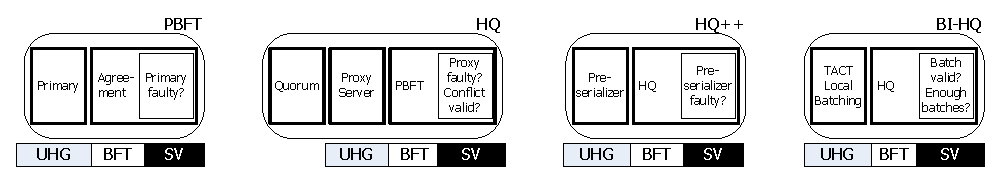
\includegraphics{visio/Examples}
%% \caption{Examples of Safe hints.
%% }
%% \label{fig:Examples} 
%% \end{figure*}

\begin{table*}
\begin{center}
\begin{tabular}{|c|c|c|c|}
\hline
System & BFT protocol & Untrusted Hint Generator & Safety Validator \\
\hline
PBFT & Agreement & Primary replica & Detection of faulty primary \\
\hline 
Q/U & ?? & Local requests & client verification \\
\hline
HQ & PBFT & Quorum \& proxy server & Proxy fault \& conflict valid \\
\hline
PS-HQ & HQ & Pre-serializer & Pre-serializer faulty? \\
\hline 
BI+HQ & HQ & TACT local batching & Batch valid \& enough batches? \\
\hline
\end{tabular}
\end{center}
\caption{Comparisons of safe hints}
\label{tab:examples} 
\end{table*}




%%%%%%%%%%%%%%%%%%%%%%%%%%%%%%%%%%%%%%%%%%%%%%%%%%%%%%%%%%%%%%%%%%%%

\section{Preserialized quorum systems}
\label{sec:preserialization}

Our first novel application of safe hints allows us to free quorum-based
RSMs from the burden of resolving contention in the absence of faults.
Our Untrusted Hint Generator is a \emph{pre-serializer} node, which
sequences client requests before they are handled by the quorum
system.  As long as the pre-serializer remains correct,
replicas never experience write contention on the same object from
multiple clients and so never have to resolve such
contention.  Hints are validated by the existing BFT mechanisms, since
pre-serializer faults are experienced by the system as write
contention or network faults. 

Our concrete example here applies the technique to
HQ~\cite{hq-replication-osdi-06} in a pre-serialized HQ protocol we
call \emph{PS-HQ}; Section~\ref{sec:ps-other} describes how
pre-serialization applies to other quorum-based RSMs. 
In the absence of significant write concurrency, basic HQ is more
efficient than PBFT, at the expense of increased overhead during high 
concurrency.  PS-HQ is able to deliver the same performance
irrespective of the level of concurrency.

\subsection{PS-HQ Design}

PS-HQ clients behave as with HQ.   

Hints are generated by one of the replicas: at any time, the hint
generator is the $i$-th replica, $i \equiv s \mod N$, where $s$ is the
current sequence number of the PBFT protocol for conflict resolution,
and $N=3f+1$ is the number of replicas\footnote{In general, a
  UHG might be chosen from the client population, or be an entirely
separate node.}.

The hint generator buffers client requests and submits them to the
HQ replicas, serially, as a regular HQ client.  Once it has received a
quorum of $2f+1$ acknowledgments (signed hashes of the request) from
distinct HQ replicas, it can submit the next serialized client
request. % batch. 

Otherwise, PS-HQ replicas behave identically to HQ replicas with one
additional exception.  They do not process regular clients' requests
immediately, but associate a timer with each one and wait for the same
request to be received from the hint generator.  If the request is
received in time from the UHG, the replica cancels the timer, sends a
grant to the client and an acknowledgment to the hint generator.  If
the timer for a client's request expires before that request is
received from the UHG, the replica initiates a hint
generator change.  
A client request that arrives at a replica after it was received from
the hint generator is ignored.

Replicas handle hint generator changes in
the same way HQ handles conflict resolution. A replica sends a
\textsc{Start} message that may contain a conflict certificate (if the
faulty hint generator submitted conflicting writes to different
replicas) or not (if the hint generator suppressed a client request
causing timers to expire).  Conflict resolution eventually results in
a PBFT invocation, which increments the PBFT sequence number and
resolves any conflicting writes.  Note that incrementing the PBFT
sequence number changes the hint generator. The cost of
changing the hint generator is similar to the cost of resolving
conflicts in HQ.

\subsection{Correctness}

A faulty hint generator appears to HQ replicas as a faulty client that
submits different requests to different replicas.  As a result, PS-HQ
shares HQ's safety properties, by relying on HQ's tolerance of an
arbitrary number of faulty clients.  

Moreover, while a faulty UHG may affect liveness by
suppressing or unduly delaying a correct client's request or batch of
requests, this eventually results in hint generator change.
Therefore, progress is ensured as long as clients retransmit their
requests until they succeed.  

Since PS-HQ relies on clients to perform the second phase of the write
protocol, a faulty client may delay writes. In HQ, if replicas receive
a new write request for an object for which there is a pending write,
they send a refusal response to the request, prompting the new client
to complete the previous request.  We use the same approach to handle
faulty clients in PS-HQ, but note that unlike in HQ, faulty clients
cannot force PS-HQ into conflict resolution by submitting different
requests with the same request identifier (RID) to different replicas 
(RID is assigned by the client to every request it sends). 

This is because in PS-HQ, requests are not given a grant at the
replicas until they are serialized.  Once serialized, a request that
encounters at a replica a disparate signed request by the same client,
invalidates the timer of that request. If a client fails after
submitting the request and before completing the second phase, PS-HQ
will time out and allows the next request to proceed (a refusal being
sent to the client of the next request). This allows the next client
to send a writebackwrite and complete the pending request of a faulty
client.


\subsection{Batching}

In the PS-HQ protocol as presented so far, the hint generator forwards
every single client request to the HQ replicas individually.  The
existence of a single hint generator affords the luxury of
\emph{batching}: instead of sending individual requests, 
the hint generator can combine multiple client
requests into a single batch, thus amortizing the cost of generating
authenticators and the bandwidth of the authenticators themselves over
many requests.  \note{Say more about how batching works; in
  particular, say something about how it replaces the fact we can't
  process things in chunks like HQ does.}

Batching does not affect the structure of the protocol but only the
number of individual messages sent: upon receiving such a batch,
replicas create a cumulative grant for the entire batch and send it to a client
chosen deterministically from the batch (e.g., the owner of the first
request in the batch).  A non-faulty client creates a write certificate
for the batch and sends it again to the replicas in phase 2.  Replicas
then send a reply message for every request in the batch to the client
who issued that request.  Note that replicas create a single grant for
the entire batch. As a result, they save both processing (by
computing a single authenticator rather than one for each included
request) and bandwidth (by sending a single grant rather than one for
each included request) proportional to the batch size. 

\subsection{Improvement Expectations}

\note{Why do we expect PS-HQ to be an improvement over HQ, and what would be
the envelope of improvement?}

The preserialization safe hint is inspired by the premise that
conflict resolution is an inherently expensive task; it 
replaces the cost of conflict resolution with the cost of
interposing a sequencer between clients and replicas that -- if
non-faulty -- serializes the request stream to remove all sources of
write contention.  The cost of conflict resolution varies among quorum
systems; for HQ, it is the cost of linearizing a conflict resolution
request via a PBFT module, which adds several replica-to-replica
communication rounds, additional authenticator computations, and some
state.  In Q/U, this is the latency cost inherent in exponential back-off,
as well as the additional bandwidth and computation for protocol message
retransmissions.

The request batching performed by preserialization should offer further
benefits, since it replaces the costs of computing and transmitting
authenticators for multiple requests with those for a single, larger
request.  In HQ's case, the benefit of batching is mitigated by the fact
that HQ's conflict resolution mechanism applies to multiple
(conflicting) requests in a single PBFT invocation.  Therefore,
preserialization without batching for HQ should \emph{reduce}
performance, since it causes every request to go
through its own protocol session (two rounds of client-replica
exchanges), whereas HQ's conflict resolution might handle them as part
of a batch.

PS-HQ batching goes beyond what HQ's conflict resolution batching can
accomplish, for two reasons. First, with regards to conflicting requests
for the same object, PS-HQ can get the same batching benefits as HQ's
conflict resolution, but at a much lower cost: a single grant and
write-2 message exchange for an entire batch, and no additional PBFT
protocol invocation over the entire batch.  Second, PS-HQ also batches
\emph{non-conflicting} requests, e.g., requests from disparate objects,
which HQ cannot relegate to its implicit batching mechanism.  Therefore,
PS-HQ improves its performance even when write contention is low but
there are high rates of requests to many objects.

Overall, at very low contention and in the absence of sustained load,
we expect HQ to be superior to PS-HQ due to the overhead of
serialization.   As sustained load increases, we expect PS-HQ
to be competitive with HQ at low contention, and at high contention
to increasingly dominate HQ, since PS-HQ's throughput is not
essentially affected by contention. 

In the presence of faults, PS-HQ's performance should be roughly
similar to HQ.  PS-HQ initiates a hint generator change, which itself
involves conflict resolution, whereas HQ simply performs conflict
resolution.  \note{Should we say more here?}

In the next section, we demonstrate this intuitive justification for the
benefits of PS-HQ experimentally.

\note{Should we add more analytical justification for the intuition,
  such as how many messages, how many round trips, etc.?}

\subsection{Experimental Evaluation}
\label{sec:eval:pshq}

We now turn to an experimental evaluation of PS-HQ.  In this section, we
show that in the absence of faults and as write contention increases,
PS-HQ maintains a roughly constant (1) high throughput, (2) low bandwidth usage,
and (3) low latency.  In contrast, HQ's throughput decreases, its
bandwidth use increases, and its request latency increases as contention
grows.

We used Emulab for our experiments. We ran experiments on 46 ``pc3000''
machines, each having a 3 GHz processor with 2 GBytes of RAM and
connected via a 1000 Mbps router. Nodes were connected in a virtual LAN.
We ran server code on 4 to 16 machines (for the number of tolerated
faults ranging from $f=1$ to $f=5$). Clients were running 4-fold on 30
machines with very low utilization, effectively 120 clients.

For a fair comparison, we used the same synthetic workload as that used
in the original HQ study.  Each client has a private object (which no
other client ever writes and, as a result, never experiences any write
contention). There is also a single object globally shared by all
clients.  Each client
has only one outstanding request at any given time; when it receives a
response to its previous request, it picks an object (its private object
or the shared one) and it generates a new request for it.  The choice of
whether to send a request to the shared or the private object is
governed by a \emph{contention parameter}: the probability that a client
will choose the shared object when sending a new request. When that parameter is set to
$0$, no request is sent to the shared object and there is 0 write
contention.  When that parameter is set to $1$, all requests are sent
to the shared object, resulting in $100\%$ contention.

\note{If we get to show multiple objects:} In another set of
experiments, we increased the number of shared objects to 10 and
100. Given a contention knob value, that fraction of requests go to one
of the shared objects. In \textit{uniform} configuration, each shared
object is equally popular.  In \textit{skewed} configuration, we have
only two shared objects and one object is 10 times more popular than the
other.

For each combination of replica group size ($4$, $7$, $10$, $13$, and $16$) and
contention parameter setting (from $0$ to $1$), we show throughput in
requests per second (computed by timing the execution of $100,000$),
bandwidth used in KBytes per request (computed by counting all bytes
sent and dividing by the number of requests), and request latency in
seconds (by measuring the average amount of time it takes for a request
to receive a response).


\begin{figure}
\centering
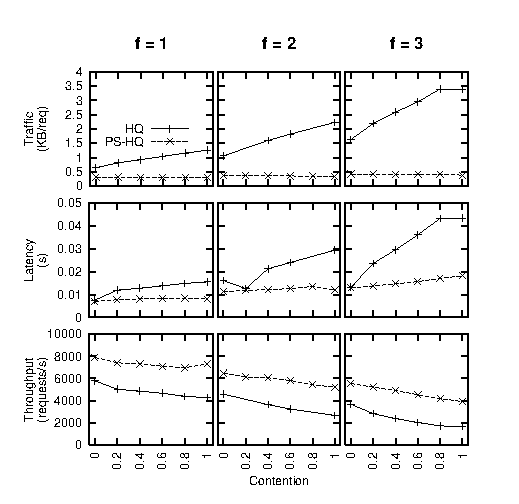
\includegraphics{graphs/ps-hq}
\caption{Throughput (bottom) measured in completed requests per second,
  per request latency (middle) measured in seconds, and traffic
  (top) measured in KBytes per request.   Contention is ranging from 0
  to 100\% on the $x$ axes. $f$ is ranging from $1$ to $3$ from left
  column of graphs to right, corresponding to replica group sizes of
  $4$, $7$, and $10$, respectively.}
\label{fig:ps-hq}
\end{figure}

\subsubsection{Comparison under HQ's synthetic workload}

Figure~\ref{fig:ps-hq} compares PS-HQ to HQ.

At low contention, the thgroughput improvement is moderate, primarily
thanks to multi-object batching.  At high contention, the improvement is
more pronounced and grows as the size of the replica group grows, from a
little under a factor of two for group size $4$ to almost a factor of
$2.5$ for group size $10$.

HQ's write throughput is always inferior compared to PS-HQ's
throughput.  

\subsection{Discussion}
\label{sec:ps-other}



\subsubsection{Other Instantiations}

\stitle{PS-Q/U} How would this work (broad strokes)?  Expected benefits?


\subsubsection{Optimization: Pipelining}

Send pre-serialized requests as they come and have the replicas buffer
them locally before executing serially. This eliminates the round-trip
time delay between preserialized request onset at the replicas.


\subsubsection{Other things to talk about if there's space and need}

From high to low priority.

\stitle{Batching vs. Preserialization} Show with batching only but not
sequencing.  Show with preserialization but without batching.  We expect
this to illuminate further where our benefit comes from: at low
concurrency from multi-object request batching and at high concurrency
from same-object batching and preserialization.

\stitle{Multiple shared objects} Homogeneous and heterogeneous access
rates.  Show that HQ does not batch conflicting requests from multiple
objects whereas we can getting further benefits.

\stitle{Different latency between clients and replicas} to be more
realistic.  Since we send fewer messages between clients and replicas,
we should be hit less by this latency and variations therein.

\if 0




\paragraph{Upper bound on throughput with PS-HQ} First, we identify the maximum attainable throughput
with PS-HQ given a throughput T with HQ protocol. For every request executed in HQ protocol, it takes
4 message delays. PS-HQ takes 5 message delays, due to the extra message between preserializer and
the other replicas. Assuming one message delay between a client and replica is represented by D$_{C-R}$
while one message delay between any pair of replicas is represented by D$_{R-R}$. Also, assume that 
message delays are symmetric. Then, HQ takes 4D$_{C-R}$ time units to complete an operation while PS-HQ
takes (4D$_{C-R}$+D$_{R-R}$) time units.  So, the drop in throughput with PS-HQ is given
by 4D$_{C-R}$/(4D$_{C-R}$+D$_{R-R}$).T. If D$_{C-R}$ = D$_{R-R}$, then PS-HQ can at best attain 4/5.T,
i.e., 80\% of HQ's throughput. On the other hand, if we assume that the delay between replicas 
is an order of
magnitude lower than the delay between replicas and clients, then
maximum attainable throughput with PS-HQ is very close to T. This is what we expect with one of our
experiments to show when we inflate the delay between clients and replicas. Also, this assumes no
contention.


\paragraph{High contention} At high contention, HQ resorts to PBFT protocol to complete
conflicting requests. At the same time, it batches multiple requests together in a single
batch, thereby amortizing the cost of PBFT protocol across such multiple requests. A graph
will show how the batching increases as contention increases. Figure~\ref{fig:hq-conflict-batch-f-1}
shows how the number of requests contained in these conflicts increase with increasing contention.
All these requests are executed at once via PBFT.
On the other hand, PS-HQ serializes these contending requests,
causing them to executed one after another. Even though PS-HQ prevents conflicts, its performance
is limited by one request execution after another. Since a request completes only after a RTT with
the client, the throughput essentially is limited by 1 request per RTT (at 100\% contention).

\begin{figure}
\centering
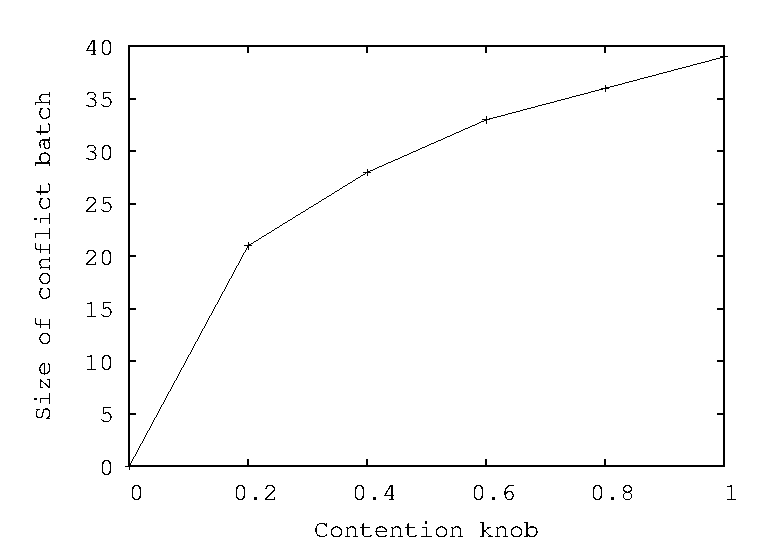
\includegraphics[width=3.0in]{temp-Figures/hq-contention-batch-f-1.ps}
\caption{Sizes of conflict resolution batches in HQ
at $f=1$.}
\label{fig:hq-conflict-batch-f-1}
\end{figure}

\paragraph{Low contention} Since PS-HQ incurs extra overhead on the preserializer replica, we
expect the performance of PS-HQ to be lower than HQ. Our results show that at no contention, PS-HQ's
throughput is much lower than HQ's, e.g., approximately 65\% of HQ. We need to identify precisely
why this is the case. 

Two experiments are done to check the hypothesis that preserializer replica is becoming the
bottleneck: (i) make one of the HQ replica perform dummy preserializer operations, e.g., send the
hint to the quorum, but nobody acts on them. They are just sent and received, and (ii) check how does
the delay in receiving a hint after receiving the request changes as the load on the preserializer 
changes.

(i) experiment shows that throughput of HQ goes down from 7400 req/s (f=1) to 5500 req/s. PS-HQ's
performance is 4888 req/s. So, it appears that the main reason of the reduction in throughput is
due to increased load on the preserializer replica. Figure~\ref{fig:throughput-compare-f-1} compares
the throughput as the number of clients in the system increase while Figure~\ref{fig:latency-f-1}
compares the average response latency observed by clients. We compare with HQ, HQ with dummy 
preserialization load on one of the replicas and PS-HQ.


Figure~\ref{fig:delay_hint} presents the average delay in receiving the hint after the client 
request has been received as the number of clients increase in the system. It shows that  as the 
number of clients increase from 1 to 80 (under no contention), the average delay in 
receiving the hint after a replica has received the write1 request grows linearly. This also supports
our conjecture that increased load on the preserializer replica is the principle reason behind the
weak performance of PS-HQ.

\begin{figure}
\centering
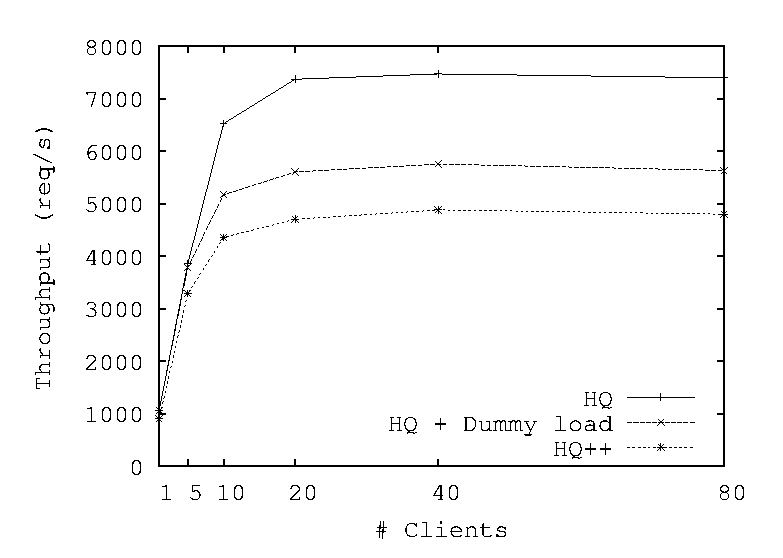
\includegraphics[width=3.0in]{temp-Figures/Throughput-compare.ps}
\caption{Comparing write throughput of HQ, HQ with dummy preserialization load and  PS-HQ 
at $f=1$.}
\label{fig:throughput-compare-f-1}
\end{figure}


\begin{figure}
\centering
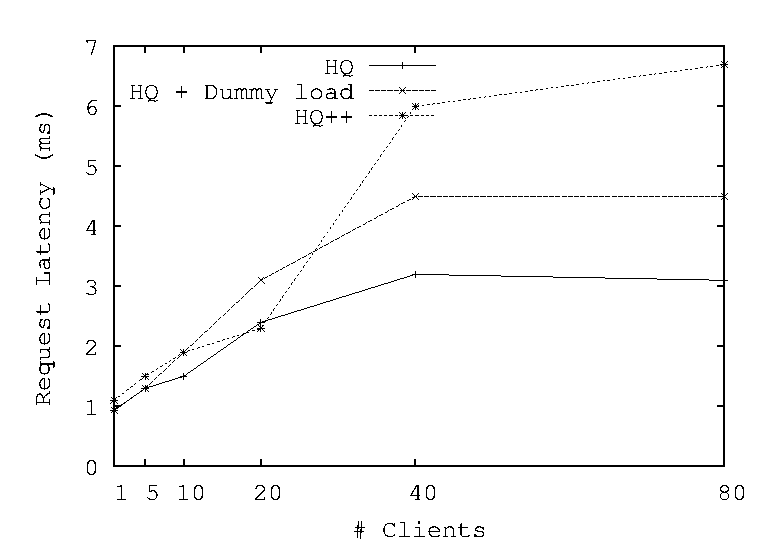
\includegraphics[width=3.0in]{temp-Figures/Latency-compare.ps}
\caption{Comparing request latency of HQ, HQ with dummy preserialization load and  PS-HQ 
at $f=1$.}
\label{fig:latency-f-1}
\end{figure}



\begin{figure}
\centering
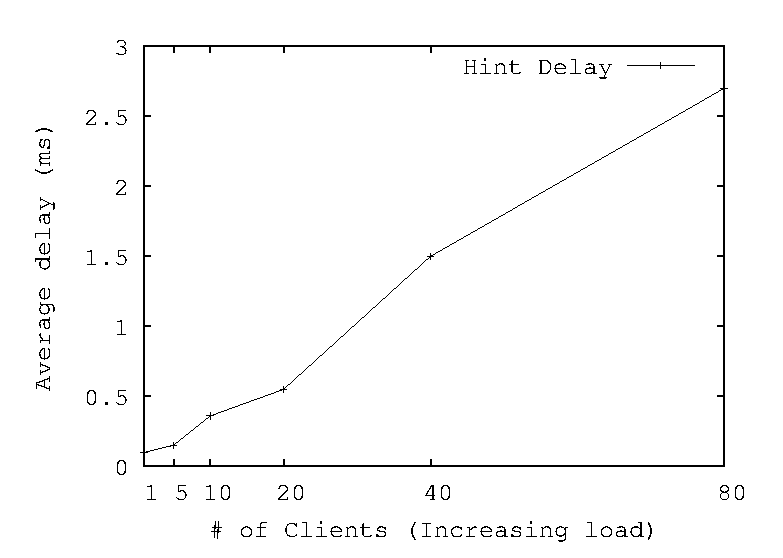
\includegraphics[width=3.0in]{temp-Figures/Hint_Delivery_Delay.ps}
\caption{Average delay in delivering the hint after the Write1 request is available at the
replicas.}
\label{fig:delay_hint}
\end{figure}


XXX: Can also potentially present the CPU utilization of preserializer replica to show the 
computation overhead and compare
it with other replicas and also HQ's replicas.

\paragraph{Multiple shared objects} Currently in our experiments, there is only one shared object. 
We now present the results when there are multiple shared objects. Given a contention factor, those
percent of requests to go to one of the shared objects. In one experiment, requests to contennding
objects are equally distributed. This would mean that HQ would need to resolve contention for different
requests independently. 



\paragraph{Higher latency between clients and replicas} Now, we emulate a network where the latency
between clients and replicas is 20ms while the latency between replicas is near zero (sub milliseconds).
This is a more realistic setting since usually clients are located far away compared to replicas which
are usually co-located in a data center. Figure~\ref{} compares the performance of HQ with PS-HQ in
this setting.

\paragraph{Scaling $f$} Here we increase the faults tolerated.

\begin{figure}
\centering
\includegraphics[width=3.0in]{temp-Figures/throughput-hq.ps}
\caption{Throughput with HQ.}
\label{fig:throughtput-hq}
\end{figure}

\begin{figure}
\centering
\includegraphics[width=3.0in]{temp-Figures/throughput-hq++.ps}
\caption{Throughput with PS-HQ.}
\label{fig:throughtput-pshq}
\end{figure}





\paragraph{Message and byte load}
Will come here.

\paragraph{Conclusion} Just serialization is not sufficient. 

\subsubsection{Batching}

Now, we introduce batching to PS-HQ. Batching helps in two different ways: (i) it reduces
the number of hints to be generated and sent by the preserializer replica, and hence reduces
 the load and (ii) protocol execution once per batch, amortizing the cost of grant creation and
certificate creation over the batch size.

Two experiments are performed. First, we simply batch the hints. Each batch contains a set of hints,
each is processed as received independently from the preserializer and HQ protocol is followed. This
will show that at lower contention, batching improves the performance of PS-HQ since it reduces the
load on the replicas, especially the preserializer. However, batching of hints does not help at
high contention since HQ is limited by the serial execution of requests. Even though multiple hints
reach at the replica at the same time, only one request will be executed at a time. 
Figure~\ref{fig:throughput-batching-hints-f-1} shows the throughput when hints are batched. 

\begin{figure}
\centering
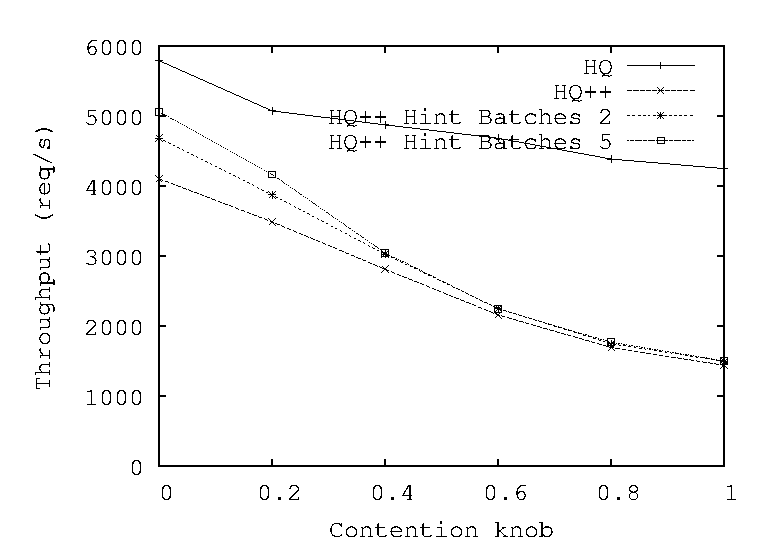
\includegraphics[width=3.0in]{temp-Figures/hint-batching-throughput-f-1.ps}
\caption{Batching of hints helps at low contention. $f=1$.}
\label{fig:throughtput-batching-hints-f-1}
\end{figure}

Next experiment will additionally implement protocol batching. This will save us the overhead in 
terms of grant creation and certificate creation. There are two different ways in which batching
can be implemented: single object batching and multiple object batching. Single object batching implies
that multiple requests for the same object can be sent in a batch. Multi-object batching allows
us to fit requests from different objects to be sent in a single batch. Single object batches have
the advantage that requests for different objects do not interfere with each other, but at low 
contention, single object batching will construct batches of very small size hence diminishing the
benefits of batching. 

Note that 100\% contention, both multi-object batching and single object-batching perform similarly
since in our experiments, we have a single shared object. Also, since at 0\% contention, multi-object
batching will outperform single object batching, we currently present only the multi-object batching
results. [XXX: single object results to appear]. Figures~\ref{fig:throughtput-pshq-batching-f-1} 
and ~\ref{fig:throughtput-pshq-batching-f-2} present the results.

\begin{figure}
\centering
\includegraphics[width=3.0in]{temp-Figures/throughput-hq++-batching-f-1.ps}
\caption{Comparing throughput with multi-object batching in PS-HQ with Hq at f=1.}
\label{fig:throughtput-pshq-batching-f-1}
\end{figure}

\begin{figure}
\centering
\includegraphics[width=3.0in]{temp-Figures/throughput-hq++-batching-f-2.ps}
\caption{Comparing throughput with multi-object batching in PS-HQ with HQ at f=2.}
\label{fig:throughtput-pshq-batching-f-2}
\end{figure}

\paragraph{Higher latency between clients and replicas}

\paragraph{Scaling $f$}

\paragraph{Cost of falling back} Now we evaluate the cost of dealing with the hint generating replica
(preserializer in PS-HQ) when it is faulty. In PS-HQ, this turns out to be pretty cheap since at worst, 
a faulty preserializer can introduce conflicts or starve some requests. First one is easily identified:
when a client sends a conflicting certificate in Write2 phase, a conflict is detected. In PS-HQ, this
can only happen when the preserializer is faulty (cite proof here). Conflict resolution is invoked
via PBFT protocol. Since preserializer replica is the replica whose id i is given by: $i = s \mod N$ 
where N is the number of replicas and $s$ is the current sequence number of PBFT protocol execution.
When the conflict is resolved, $s$ advances and hence preserializer changes automatically. Figure~\ref{}
shows the cost of switching the preserializer when it introduces conflicts.

Next, starvation is detected by starting a timer when the request is received. If the timer expires 
before a hint is received for the request, replica first sends the request to the preserializer and
restarts the timer. If the timer expires again, replica initiates a preserializer change by invoking
a dummy conflict resolution via PBFT. Once PBFT completes, preserializer changes.




\fi













































\section{Bounded Inconsistency for Replicated State Machines}
\label{sec:boundedInconsistency}

Relaxing consistency is a widely used technique to improve the
performance of replicated
systems~\cite{Satyanarayanan2002,Terry1995,Yu2002} with non-Byzantine,
crash faults.  Applications that can tolerate bounded inconsistency 
trade consistency for significantly reduced latency and, in some cases, increased throughput. Example
classes of such applications are, for instance, compliance enforcement
systems (e.g., quota enforcement, resource sharing fairness), risk
management systems (e.g., banking applications, airline reservation and
crew scheduling applications, etc.), and monitoring systems (e.g.,
enterprise network anomaly detection).  BFT RSMs have been traditionally
avoided in these settings, due to their high per-request costs.

In this section, we build a Byzantine-fault
tolerant bounded-inconsistency mechanism  (or \emph{BI-BFT}) that follows the safe hints
pattern and works for any BFT RSM that provides linearizability.  We
describe this mechanism in the context of Castro and Liskov's PBFT,
which we call BI-PBFT.  The same approach works on top of other BFT
RSMs; we have implemented and show results for BI-HQ and BI-PS-HQ, and
we have designed BI-Q/U as well but have no access to the source code to
evaluate the performance improvement from our safe hint.



\stitle{TACT Background} For the purposes of BI-BFT in this paper, we
focus on bounded-inconsistency systems in the vein of the \emph{Tunable
Availability and Consistency Tradeoffs} (TACT) project by Yu et
al.\cite{Yu2002}.  TACT provides a framework for applications to specify
their consistency requirements for accesses in a fail-stop replicated system.  A
replica may tentatively reply to a client request immediately, before
that request is committed to all replicas of the system's
state. Therefore it may produce an inconsistent result.  Applications
specify an acceptable consistency bound using different metrics. For
instance, a numerical error metric is defined to be the \emph{weight} of
updates that the inconsistent, tentative result to an operation could
miss, compared to what it would have otherwise seen in a strictly consistent
(linearized) execution; the weight function $F$ is application-specific and
is defined as part of the application's basic consistency unit (or
\emph{conit}, in the terminology of TACT).  To illustrate with an example, consider an airline
reservation system in which bumped customers of overbooked flights
receive a compensation.  A weight function for every reservation request
would be the compensation that the airline would owe the passenger if her reservation
could not be honored due to overbooking.

In TACT, inconsistency is \emph{bounded}, since replicas give a
tentative reply to a client's request only if that reply's
inconsistency is guaranteed to be within a given bound.  In the
airline example, the bound could be the airline's total budget for
compensations due bumped customers.

In crash-fault environments, TACT provides bounded inconsistency with regards to
numerical error by allowing each individual replica to locally process clients' requests, as
long as the total weight of those tentative requests does not surpass a local bound
$\beta$. When a new request arrives that could cause that bound to be
violated, the replica propagates its updates to all other replicas
synchronously before tentatively replying to the newly arrived
request.  The global numerical error bound $\alpha$ is set by the
system administrator; the local-replica bound $\beta$ is derived from
$\alpha$ and the number of replicas in the system. In TACT, $\beta=\alpha/(N-1)$, where
$N$ is the number of replicas.







\subsection{An Example: BI-PBFT}
\label{sec:bipbft}

BI-PBFT brackets Castro and Liskov's PBFT RSM with a
bounded-inconsistency safe hint. BI-PBFT replicas act as clients of the
PBFT RSM, proxying end users' requests. We refer to BI replicas and PBFT
replicas as separate entities, but in practice they are likely to run on
the same physical machine.  For simplicity, we only consider numerical
error in this paper.

\subsubsection{Design}

\stitle{The Synchronization Object State Machine} BI-PBFT creates one
synchronization object for every set of client objects forming a single
consistency unit.  For instance, if BI-PBFT is used to ensure that
updates to a single object are bounded in their inconsistency,
independently of other objects, then a single synchronization object is
created for each client object.  In another example, if BI-PBFT is used
to ensure that updates to any object are globally subject to a single
inconsistency bound, then a single, global synchronization object is
used for all client objects.

A synchronization object is managed by a state machine that is executed
reliably by the replicated state machine protocol, PBFT in the current
design.  The state of the synchronization object consists of a single
log of \emph{Synchronization Sets} corresponding to client objects
subject to that synchronization object.  Each synchronization set
contains up to $2f+1$ request batches, each submitted by a distinct BI
replica.

The synchronization object has two operations:
\method{append}$(\mathit{ReplicaID}, \mathit{ClientRequestBatch})$
returning a $\mathit{SequenceNumber}$, and
\method{synchronize}$(\mathit{SequenceNumber})$ returning a
synchronization set made of all $2f+1$
$\mathit{ClientRequestBatch}$es in the synchronization set with that
sequence number.  \method{append} is a write operation whereas
\method{synchronize} is a read-only operation.

Intuitively, a synchronization object allows BI replicas to append
client operation batches to the current synchronization object, ensuring
that (i) each client operation batch does not violate the local $\beta$
bound on the cumulative weights of all included client operations, and
that (ii) no synchronization set contains more than one batch from each
replica.  When a synchronization set fills up, a new, empty set is
appended to the log and starts accepting client request batches in
subsequent \method{append} operations.  \method{synchronize} operations
for a synchronization set that is not yet full or has not even been
created return a distinguished null synchronization object.
























\stitle{Clients} An end client sends a request to all BI nodes and waits
for $2f+1$ matching replies before considering the request
$\emph{completed}$.  The client maintains a timer for each pending
request. If the timer expires, it retransmits the request.


\stitle{Replicas} Each BI replica -- acting as the UHG in the safe hints
pattern -- is a PBFT client.  For each consistency unit, a BI replica
maintains a list $T$ of tentative client requests that it has received
and tentatively responded to since the last synchronization, the last
synchronized service state and the largest request timestamp it has
processed for every client.


\stitle{Client request handling} When a BI replica receives from client
$c$ a new request (with a timestamp larger than the largest known
timestamp by client $c$)\footnote{A request with an earlier timestamp
than the latest seen for that client is treated as a retransmission and
may be handled using a local cache. We omit the (straightforward)
details here for brevity.}, it ensures that this new request, if
tentatively executed, would not cause it to violate its local
inconsistency bound $\beta$ (see below).  Then, it appends the request
to its buffer $T$ for the corresponding consistency unit (determined
uniquely by the object involved in the request) and produces a tentative
reply based on its local state, to which it applies all tentative
requests in $T$ sent by client $c$.  It returns to client $c$ the
computed result $r$ in a tentative reply message.


\stitle{Error bounding} A BI replica checks if the inclusion of the new
client request into the tentative requests $T$ would cause neither the
total positive weight nor the total negative weight of tentative
requests to exceed a threshold $\beta$. If so, then error bounding is
complete and the replica can continue handling the request to issue a
tentative response from its local service state.

Otherwise, the BI replica invokes an \method{append} method on the
corresponding synchronization object via PBFT, with a client request
batch made up of its tentative requests in $T$ (excluding the newly
arrived request).  Once the replica receives a response to its
\method{append} method with some sequence number $s$, it invokes a
\method{synchronize} method with that sequence number $s$, which it
repeats until it receives a non-null synchronization set back.
Until then, 
the replica queues  the offending client request and
any future received requests.



Once the replica obtains a non-null synchronization set back for its
most recent client request batch, it executes all included client
requests contained within (ignoring duplicate client requests) in some
deterministic order on its service state.  Afterwards, it can unblock,
flush its buffer $T$ of tentative requests, begin
processing further client requests from its queue or the network.








\subsubsection{Safe Hint Organization}



\subsubsection{Guarantees}

As with TACT, the BI-PBFT protocol guarantees that the result of a
completed request can at most miss updates of weight $\alpha$ that it
would have otherwise seen in the system's linearized request ordering.
BI-PBFT is also live: it ensures that a non-faulty client eventually
gets its pending requests completed.
Submitted requests that are not completed -- that is, for which the
client does not receive $2f+1$ tentative, matching replies -- \emph{may} eventually
be committed, but no guarantee is given
on any tentative reply value; the client will eventually retransmit the
request and receive matching replies that may be tentative or committed,
depending on whether the original request was not committed at all.


\iffalse
Restricting tentative requests to receiving replies based only
on the same client's tentative requests s ensures that the client
receives ``read your writes'' session guarantees on its own tentative
requests between checkpoints.
\fi






\subsubsection{Informal Correctness}

For safety, first we need to ensure that $2f+1$
valid BI batches contain requests of at most $\alpha$ weight. Second, we 
need to show that every completed request appears in at least one of the $2f+1$
valid batches. We ensure the first property by observing
that BI replicas request synchronization
once they have collected requests of weight $\beta$ in a BI batch.  Replicas
only commit requests in the local state when BI batches from $2f+1$ unique replicas 
have been committed by HQ. Let these replicas form a quorum $Q$.  Setting
$\beta=\alpha/(3f+1)$, we are ensured that the weight of requests
contained in these BI batches is bounded by $\alpha$. 
By definition of a
completed request, at least a quorum of $2f+1$ replicas responded,
call it $P$. By the quorum intersection property, at least one
non-faulty replica is common to $P$ and $Q$ and the completed request
appears in that replica's BI batch. Hence, the second claim holds. Our safety
guarantee, i.e., the numerical error seen by a completed request is bounded by $\alpha$, 
follows from these two claims.
% Hence, our safety guarantee of bounding
%the numerical error of a completed request by $\alpha$ follows.
For liveness, we have to ensure that BI replicas do not wait indefinitely
to complete the synchronization round. 
BI replicas associate a timer with the synchronization requests. If the timer expires
before the synchronization round completes, the BI replica multicasts its list $T$ of 
requests to other replicas. This ensures that other non-faulty replicas would also initiate
the synchronization and complete the synchronization round.










\subsection{Improvement Expectations}

The big win with bounded inconsistency comes from the ability of a
replica to unilaterally return a tentative response immediately upon
reception of a request -- as opposed to after a costly commitment
protocol that synchronizes all replicas to the latest, common service
state -- and yet guarantee a bound on the error of that
tentative response.   The longer a replicated state machine takes to
reach ideal consistency (5 message delays for PBFT's 3-phase protocol, 4
message delays for HQ's 2 phase protocol, longer for conflict
resolutions, view changes, etc., with either), the bigger the savings in
latency that clients experience when they can tolerate the
inconsistency.

Our bounded inconsistency protocol offers another source of potential
performance improvement with regards to throughput. In the general case,
BI is a form of request batching and, as a result, it can amortize the
cost of the replicated state machine protocol over many bundled
requests.  However, there are some requests that an RSM such as PBFT
could not possibly batch together whereas BI can: those are successive
requests from the same client to the same object. In an ideally
consistent RSM, such requests cannot be in the same batch; the first
must be completely linearized and executed, giving the client a reply,
before the client can submit the next.  Clients in BI-BFT are no
different; however, an RSM commitment is not required before a
(tentative) reply is
sent back to a client. So multiple successive requests can be buffered
at a replica, before it will push its BI batch to the RSM for
synchronization.

The major cost of bounded inconsistency comes from message duplication
due to its two-tiered structure: a client multicasts a request to all BI
replicas which, eventually, will each submit that request as part of a
BI batch to the RSM.  In the strawman BI protocol we have described,
this means that every client request is transmitted over the wire $N$
times from a client to all BI replicas, and then $N$ more times in the
worst case from each BI replica to the RSM.  The size of individual
requests and the degree to which the deployment is bandwidth-constrained
can determine how significant this duplication can be.

Therefore, we expect BI-BFT to yield lower average latency as the number
of requests that can receive tentative responses within a round-trip
time increases -- the higher the tolerable inconsistency, the more such
requests are handled tentatively before a synchronization must occur.
Furthermore, the greater the latency cost of an RSM
operation compared to the latency between clients and replicas, the
bigger the average latency reduction for a given inconsistency bound and
workload.

With regards to throughput, we expect BI-BFT to perform better for
workloads in which larger batches are possible than in an ideally
consistent RSM.  For instance, workloads with relatively few clients
with many successive requests would limit
a batching RSM to batches of size equal to the number of clients,
whereas BI-BFT with a high inconsistency bound might be able to commit
to the RSM at a much lower frequency, amortizing RSM costs over many
more requests.








\subsection{Experimental Evaluation}

We use the same experimental setup as with Section~\ref{sec:eval:pshq}.
The
workload we use consists of a single object within the consistency unit
shared by all clients.  Each client request has weight of $1$.
Therefore, a BI replica can buffer requests and respond tentatively as
long as it has fewer than $\beta$ requests in its tentative request
buffer $T$.

We perform experiments with increasing inconsistency bound, and with
increasing numbers of clients, to explore the differences in throughput
due to sequential client requests between PBFT and BI-PBFT.
Figure~\ref{fig:bi-pbft} shows that throughput increases as the number
of clients increases, and reaches a plateau past 25 clients.  As the
consistency bound increases, so does the throughput.

\begin{figure}
\centering
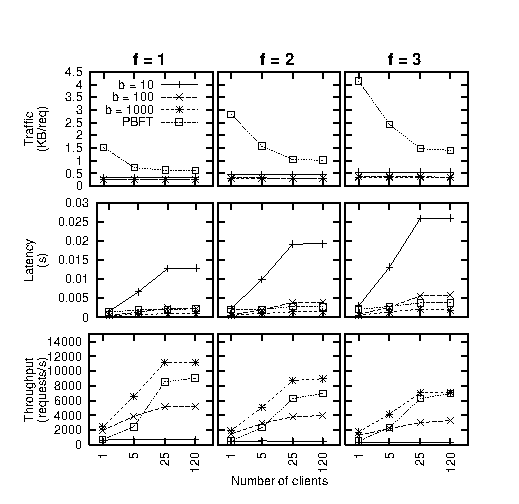
\includegraphics{graphs/bi-pbft}
\caption{BI-PBFT. Throughput (bottom) measured in completed requests per second,
  per request latency (middle) measured in seconds, and traffic
  (top) measured in KBytes per request.}
\label{fig:bi-pbft}
\end{figure}

A noteworthy artifact of our BI design above can be observed with
regards to the $\beta = 10$ lines on the throughput graph.  BI replicas
send in their BI batches
\emph{only} requests to which they have tentatively replied, even if
there are pending requests in their overflow queue.  PBFT's
opportunistic batching might linearize and execute all pending requests and provide an
ideally consistent response to clients in the amount of time and work
that it take BI-PBFT to synchronize its tentatively executed requests,
only to take another batch in the next iteration.  A simple
optimization that hybridizes BI batches to contain not only requests for
which tentative replies have been produced (filling up the $\beta$
bound) but also all remaining pending, unanswered requests appears in
the Discussion section. In this section, we opted for the cleanest
version of the BI safe hint, that demonstrates that indeed, there is an
envelope of parameters (high $f$, high $\beta$) for which BI-PBFT
dominates PBFT.

In contrast, the ``PBFT'' plot on Figure~\ref{fig:bi-pbft} presents the
results for the PBFT protocol with minimum batch size of $10$ (higher
batch sizes did not improve throughput). Compared to BI-PBFT, PBFT achieves better throughput, lower
latency and lower traffic overhead when numerical error is on the order
of a few hundred. At lower
numerical error, PBFT is superior. This can be explained due to the fact that our BI-PBFT protocol 
needs to block while the commit phase commits. Also, during the commit phase, each replica
submits its buffer of tentative requests to the PBFT layer independently, causing a quadratic number
of message transfers. At lower values of numerical error, commit happens more frequently and hence
BI-PBFT blocks more frequently causing BI-PBFT's throughput to drop significantly. Also, increasing
the number of clients does not help BI-PBFT at all since commits happen at the rate of $\beta$ and
it is immaterial which client requests fill up the buffer. However, PBFT's performance improves as
the number of clients increases since it is able to perform batching of the requests as well
as pipeline multiple batches in parallel. 

At high values of numerical error, BI-PBFT is superior since it incurs commit infrequently, at a rate
determined by $N/\beta$. While the tentative buffer fills up, replicas respond immediately to the
requests, providing a reduced latency to operations. One artifact of our experimental setup is that 
the latency between any pair of nodes is near zero. So, multiple rounds of PBFT protocol do not affect the
latency of PBFT significantly. However, in a real setting, the delays would be in the order of few
milliseconds and multiple rounds of PBFT will incur more delay compared to BI-PBFT.

\if 0
\begin{figure}
\centering
Placeholder.
%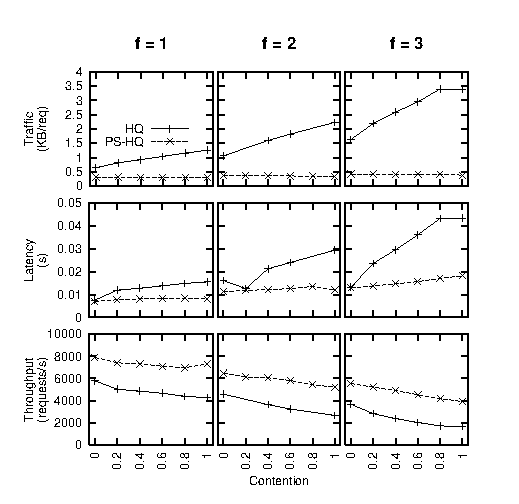
\includegraphics{graphs/ps-hq}
\caption{BI-PBFT. Throughput (bottom) measured in completed requests per second,
  per request latency (middle) measured in seconds, and traffic
  (top) measured in KBytes per request.}
\label{fig:bi-pbft-increasedLatency}
\end{figure}

We also perform experiments with increasing point-to-point latency, to
explore how the relative cost of RSM operations to communication between
BI replicas and clients affects average latency (Figure~\ref{fig:bi-pbft-increasedLatency}).
\fi




\subsection{Discussion}


\subsubsection{Envelope}
Our results show that when consistency in terms of the numerical error is relaxed only slightly, BI-PBFT
performs worse compared to the strict consistency provided by the PBFT protocol. This raises an interesting
question: Is relaxing consistency in the BFT domain helpful and is it worth the complexity? 
We believe that the answer is in affirmative.
This is because of at least three reasons. 

-First, BI-PBFT is being compared with the PBFT protocol that has
been optimized significantly over years of research and via specialized engineering techniques 
such as pipelining and batching. On
the other hand, our implementation and design is a first instance of a weak consistency protocol that is able
to tolerate Byzantine faults.

-Second, even though BI-PBFT's performance is worse compared to the PBFT protocol, it neverthless
shows that when an application is able to tolerate large errors in the responses, BI-PBFT is infact superior.
Fine tuning of the implementation as well as the protocol may help us in getting the cross-over to happen
much quicker than what the current results show. In the next section, we enumerate a set of optimizations
that will improve the performance of BI-PBFT.

-Last but not the least, we have not yet introduced message
delays and loss in the system, which will invariably introduce performance problems for the PBFT since it needs
to communicate with other replicas multiple times before it can respoond. BI-PBFT, on the other hand, does not
have that limitation. 


\if 0
\subsubsection{Other Instantiations}

The design of BI-HQ and BI-PS-HQ is identical to that of BI-PBFT, with
the substitution of HQ and PS-HQ as the RSM, respectively.  Because the
BI synchronization object is written by multiple BI replicas during each
synchronization, we expect BI-HQ to perform worse than BI-PS-HQ, since
the former must frequently perform conflict resolution operations.

We show results for both instantiations here.


\begin{figure}
\centering
Placeholder.
%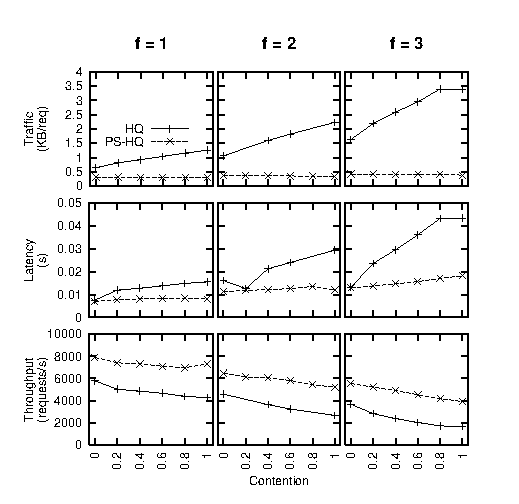
\includegraphics{graphs/ps-hq}
\caption{BI-PS-HQ. Throughput (bottom) measured in completed requests per second,
  per request latency (middle) measured in seconds, and traffic
  (top) measured in KBytes per request.}
\label{fig:bi-hq}
\end{figure}

\fi

\subsection{Potential optimizations}

Below we list the set of optimizations that can be potentially applied to the BI-PBFT protocol.


\subsubsection{Optimization: Hybrid BI Batching}

In our current implementation, BI-PBFT replicas only commit requests that they
have tentatively responded. However, as number of clients increase, request queue
at the replicas will grow while the previous commit operations finishes. A simple
optimization is to also append the set of requests that a replica has \emph{not}
responded during the next commit event if available. 


\subsubsection{Optimization: BI Batch Preintegration}

The BI safety hint can be further refined to improve the performance of
BI-BFT under fault free settings. Note that BI-BFT, as described in 
Section~\ref{sec:bipbft}, requires $2f+1$ RSM protocol invocations to 
complete the synchronization round. With the pre-integration hint, we can reduce
the PBFT invocations to just one. We now explain the modified synchronization round 
(all other aspects of BI-PBFT remain unchanged).


Once a replica locally receives tentative requests of weight $\beta$ (a
BI batch), it informs a distinguished hint
generating (UHG) replica and starts an associated timer. 
The hint generator replica then waits for $2f$ other replicas (including
its own) to submit their BI batches (each with weight less than $\beta$), and then
invokes the PBFT protocol with a request formed by pre-integrating these BI batches.
Once the RSM  linearizes the request, the SV module verifies the correctness of the pre-integration
hint as with BI-PBFT. If correct, the requests contained
in the BI batches are executed in some deterministic order immediately
(that is, it is no longer necessary to wait for $2f+1$ BI batches one at
a time to be linearized), marking completion of the synchronization
round. If incorrect, the UHG is changed and synchronization is
retried. If the timer expires before
the synchronization round is complete, a replica submits its tentative batch to all other replicas,
causing them to invoke the synchronization round and a possible UHG change.

\stitle{Informal correctness} The safety property (i.e., consistency bounds are guaranteed) follows
directly from the arguement for the safety of BI-HQ protocol since replicas do not complete
the synchronization round unless they have seen $2f+1$ BI batches each with requests of weight less 
than $\beta$.  A faulty UHG may however affect the liveness
by not invoking the HQ protocol even after receiving a quorum of BI batches. This is not a problem
since the timers at the non-faulty replicas will expire, causing a UHG change.

\subsubsection{Preserialization}

In Section~\ref{sec:pshq}, we showed how preserialization improves the performance of quorum
protocols by avoiding the conflicts. Same idea can be applied to the BI-PBFT protocol and we
explain it briefly here. All requests are preserialized by a preserializer replica and each BI-PBFT
replica tentatively responds to the requests that have been serialized. The advantage here is that,
as long as the preserializer replica is non-faulty, all non-faulty replicas will have identical tentative
requests in their buffer. When $\beta$-weight of requests are received by the replicas, only the 
preserializer replica needs to commit, avoiding each replica to commit independently.


\subsubsection{Optimization: Duplicate Request Elimination}

Only submit request IDs and only send actual requests once.





\section{Protocol Adaptation}
\label{sec:protocolSwitching}

In our last safe hints application, we describe a mechanism for safely
tuning the operating parameters of a BFT RSM to changing workloads or
application needs.  Such operating parameters might be timeouts and minimum
batch sizes in PBFT, or whether to use preserialization in HQ.  The hint
generator proposes such a tuning action (e.g., ``turn on
preserialization'') and the safety validator executes it as long
as the verification criterion on the hint is fulfilled.

We show below two mutually complementing concrete examples, a safe hint
that can heuristically lead an HQ system to turn on preserialization,
becoming PS-HQ, and the converse safe hint that can lead a PS-HQ system
to turn off preserialization, becoming HQ.  As we demonstrated in
Section~\ref{sec:preserialization}, HQ has higher throughput than PS-HQ
under very low concurrency, whereas PS-HQ performs better under high
concurrency.  This suggests that choosing whether to use PS-HQ according
to current levels of concurrency may improve performance overall.




\subsection{HQ To PS-HQ}

In our first example, HQ replicas track the heuristic criterion that, if within
the last $k$ committed requests more than a fraction $c$ of them have been
relegated to conflict resolution, the system should switch to preserialization.
When a replica believes this criterion true -- when the replica
is about to request the HQ conflict resolution that makes the criterion
true -- it submits its hint along with HQ's \msg{Start} message, as an
extra field of the message format.  The safety validator for the hint
executes within HQ's conflict resolution state machine (within PBFT):
once the conflict has been resolved, if at least $f+1$ of the \msg{Start} messages
in the conflict request contained the hint, then the resolution
state machine decides to switch preserialization on.  As soon as a
replica receives an update from the conflict resolution state machine
that the conflict has been resolved (and preserialization has begun), it
starts executing PS-HQ as opposed to HQ.

Upon the switch, any client requests past HQ's
phase-1 complete unhindered, potentially through an additional conflict
resolution.  Subsequent client requests must be preserialized as per
PS-HQ.



\subsection{PS-HQ to HQ}

The complementary example of the switching safe hint has a similar
structure.  To switch from PS-HQ to HQ, the heuristic consists of
checking the number of successive preserialized request batches 
containing requests that, without preserialization, would have created
conflicts.  When fewer than a fraction $c$ of the last $k$ request
batches contain conflicting writes, a replica issues a hint to switch
back to HQ.  The hint is conveyed, as above, in a conflict resolution
request (a \msg{Start} message) that contains an empty conflict set, and
a hint in an extra message field.  The proxy server collecting
\msg{Start} messages only begins a conflict resolution with PBFT when it
has received $2f+1$ such messages.  Then the conflict request has been
linearized, the safety validator for the hint checks that at least $f+1$
of the \msg{Start} messages contain the hint.  If so, the replicas
executing that request switch back to HQ.

Upon the switch, any pending request batches that are already
past phase-1 of HQ will complete unhindered. Preserialized
requests arriving at a switched replica are ignored.
Client requests buffered at a switched replica are handled immediately,
as if they just arrived from the client. 

In both switch directions, non-faulty replicas that did not participate in the PBFT quorum
committing the switch find out about the switch during regular PBFT
state transfers (aimed at bringing lagging replicas up to speed with the
committed history of the system).



\subsection{Improvement Expectations}

Unlike the previous safe hints we have described in this paper, the
direct cost of the protocol adaptation safe hints we presented is very
low: from HQ to PS-HQ, the cost is merely that of conveying an extra bit
along with a conflict resolution message at a quorum of replicas.  From
PS-HQ to HQ, the cost is that of a conflict resolution invocation
through PBFT.  Indirect costs are tantamount to premature or delayed
switching, in the form of missed benefits, and in wasted effort for
preserialized requests that are dropped due to a switch back to HQ.
Hysteresis (effected via the setting of the switching sliding window
size) can mitigate such wasted bandwidth and computation costs.

A workload scenario in which our switching safe hint may cause
degradation over using either of the two protocols exclusively is one in
which switching in protocols and applicable workloads is in perfect
synchrony but out of phase.



\subsection{Experimental Evaluation}

We construst a scenario in which the system workload characteristics go
in and out of the envelope in which preserialization is beneficial.
Specifically, in our experiment, the delay between successive requests
by the same client varies between $0$ and $20$ ms.  When the request
rate is low, PS-HQ suffers due to batching, effectively submitting
requests at the rate of its batching timeout expirations.  Instead, when
the request rate is high, PS-HQ always manages to collect large enough
sets of requests to justify transmission without waiting, realizing its
benefits.

\begin{figure}
\centering
Placeholder.
%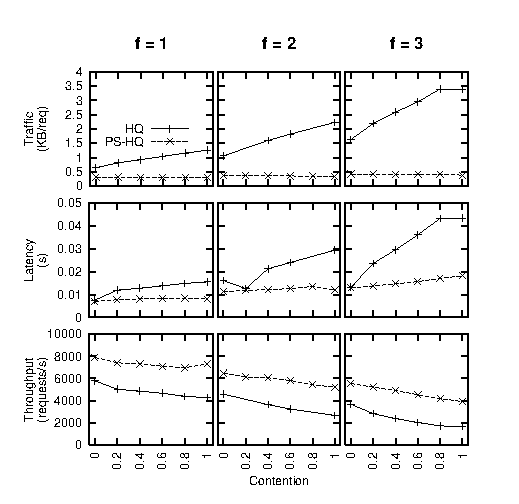
\includegraphics{graphs/ps-hq}
\caption{Switching between PS-HQ and HQ. The $y$ axis contains
  instantaneous throughput (computed at 1-second sliding windows) and
  the $x$ axis shows time.}
\label{fig:pshqswitcher}
\end{figure}

In Figure~\ref{fig:pshqswitcher}, we plot HQ, PS-HQ, and Switched-PS-HQ
for the same workload scenario, starting with low request rates at time
$0$, jumping to high request rates at time $300$ sec, and dropping back
down to low request rates at time $600$ sec.  The throughput of
Switched-PS-HQ is roughly that of the upper envelope of the throughput
for HQ and PS-HQ.


Vary the rate at which the scenario switches back and forth.



\subsection{Discussion}





\section{Divide and conquer}

Goal is to reduce the protocol overhead at high $f$. We partition
the replicas into two disjoint groups of half the sizee. Each replica still maintains the 
full system
state and executes every operation. However, only a group is responsible for the
protocol execution of requests updating or reading half of the system state, which 
we assume is composed of multiple objects (neglect transactions for now). 
Assume the system size is N and it can tolerate upto 1/3rd faults, F
(N $\ge$ 3F+1). By partitioning, we have 2 groups of size N/2. First, let us describe how the
system works. 



\paragraph{Insight} PBFT protocol can be configured for different guarantees between safety
and liveness. For both safety and liveness, we know that N $\ge$ 3F+1. But we can tolerate
more faults by trading off  liveness. For example, we can tolerate
upto 2/3rd faults and still provide safety but liveness is lost as soon as more than 1/6th 
of the replicas fail. This means that we can optimistically partition
the replicas into two groups and make each group ensure safety (at most
2/3-rd of the replicas can fail in any group of half the system size in this setting when system as a whole
has F faults) but trade liveness. When
we suspect that liveness is lost (timeouts), we fall back to the PBFT of the whole group and
that is guranteed to be safe and live. 

\paragraph{Assumptions} \note{Use of asymmetric crypto -- check this}. Each request identifies which group will
process it.  N is the system size and $F$ is the maximum number of faults that can occur
simultaneously in the system. G is the group size and $g_l$ represents the maximum number of faults
that does not affect liveness while $g_s$ represents the maximum number of faults that does
not affect safety. Note that $g_l=G/6=N/12=3F/12=F/4$ and $g_s = 2G/3=F$. So, safety is guaranteed
even when all faults occur in the same group. However, it is possible that both groups are not live.
Quorums are of size $Q_G=5/6.|G|$, where $|G|$ is the group size

\paragraph{Client access protocol} A client submits the requests to the whole system and considers
a request completed as soon as it receives $F+1$ matching responses. A client is not aware of the fact
that the system implements divide and conquer safe hints.


\paragraph{Replica Protocol: Intra-group} Primary of the group responsible for handling a request 
will propose an ordering (using Pre-Prepare message) to the requests using the PBFT protocol, with $Q_G$ as the quorums. Once a non-faulty replica has received a quorum ($Q_G$) of matching Prepare messages, then it participates in the commit phase
by sending a COMMIT message to the other replicas of its own group. Once a quorum $Q_G$ has sent a COMMIT,
a replica enters the execute phase. In this phase, the replica notifies the other group of the request that committed. 
It then waits for an ACK from (G/2+1) members of the other group and 
participates in the Inter-group protocol to notify the other group. Once a non-faulty replica receives an
ACK from (G/2+1) members of the other group, it commits the request and sends the response to the client. 


\paragraph{Replica protocol: Inter-group} Inter-group protocol is necessary to ensure that when one or both
groups loose liveness, then the whole system is able to make progress by identifying the requests that committed
in each group. Just like the original view change protocol, as long as each committed request is present in at least
$2F+1$ replicas, we are guaranteed to collect such committed requests. Now, let us describe in detail how inter-group protocol works.
Suppose replicas from group G1 need to commit requests. Each replica in G1 sends a COMMIT message to every
replica in the group G2. Replicas in G2 do not respond immediately, in fact, they wait to see a quorum $Q_G$ of matching
COMMIT messages before they send the ACK. Replicas in G2 store such COMMIT messages. 
Replicas in G1 wait for $k$ such ACK messages, where $k+5/12.N \ge (2F+1)$, i.e., a total of $(2F+1)$ replicas should see a 
given COMMIT message. This gives $k\ge\lceil G/2 \rceil+1$.


\paragraph{Liveness recovery phase} Each replica starts a timer when it receives a message. If the timer expires before the
request is executed, then it needs to take a corrective action. When a
non-faulty replica suspects that liveness is lost (timers expire), it broadcast a NEED-N-PBFT(v+1), where v is the current
view for the N-PBFT protocol. Primary of the N-PBFT
protocol waits to hear matching such messages from at least (F+1) replicas before it initiates the liveness recovery phase. Essentially,
this phase is similar to the view change protocol: the primary need to identify the requests committed by the two groups after the last
stable checkpoint. Since non-faulty replicas notify a quorum of (2F+1) replicas about the requests that committed in their groups, at 
least one non-faulty replica would be able to notify the new primary about every such committed request.   


\paragraph{Where is the gain?} As long as the number of real faults in the system is less than F/4 in each group,
each group is both safe and live. In that situation, the message load per request is given by: pre-prepare sent to 
G1 (equal to G1 messages), broadcast of prepare by replicas in G1 (equal to G1*G1 messages), broadcast of commit by
replicas in G1 (equal to G1*G1 messages), broadcast of COMMIT
by replicas in G1 to replicas in G2 (equal to G1.G2) and broadcast of ACK from  replicas in G2 to replicas in G1
(equal to G1*G2). Assuming G1=G2, the overall cost of the protocol is $G+G.G+G.G + 2.N/2.N/2=N/2+N.N$. The cost of using PBFT over the whole group is $N+N.N + N.N=N+2.N.N$. So, the reduction in number of messages is 2.

Note that the size of each of these messages is constant (none of them contains a certificate), hence the reduction
in byte sizes is also 2.

\paragraph{Why is it a safe hint?} Because it improves performance when actual faults experienced are small in
comparison to the worst case without compromising the safety.

\paragraph{Safety} For safety, we need to ensure that a non-faulty replica only responds when a quorum $Q_G$ of replicas agree. 

\paragraph{Liveness} We can not guarantee that each group will be live. To ensure that recovery phase is live, we have to ensure that each committed operation of any group
is present in at least a quorum $Q_N$ of replicas (=2F+1). 

\paragraph{Frequency of liveness recovery} As long as the number of faulty nodes in a group is less than G/6, it is live. 
However if the primary is the only faulty replica, then we may have to resort to view change to change the faulty primary.
So, in this fault zone ($0 \le g_l \le G/6$), view change
is beneficial rather than falling back to the N-PBFT protocol. As the number of faults increase, the view change protocol in the group
may not terminate and hence we may have to fall back to the N-PBFT. However, falling back to the N-PBFT incurs the additional cost of 
collecting the commit requests. So, frequently switching back and forth between group PBFT and N-PBFT may be expensive. We can
envision another safe hint where replicas do not switch back to the group PBFT if they suspect the number of faulty replicas in a group is
more than G/6, sort of the protocol switcher.





























\section{Speculative Execution}

Goal is to reduce the response latency. Each replica,
upon receiving the request, sends the grant and piggybacks a tentative response. If a
client receives a quorum of matching grants as well as matching responses, then it
may accept that response as the early, tentative response. Note that under no
contention, this tentative response will be the final, committed response. As long as the
pre-serializer replica is non-faulty, there will be no contention and hence the 
tentative response would be a committed response. The benefit is that the response latency
drops to one RTT to a quorum of replicas.


Clients still
need to participate in the write back, and replicas still need to participate in the
second phase. 

















































\section{Related Work}

Safe hints are also related in spirit 
to speculative techniques used in other types of systems, including
distributed systems~\cite{Speculator-sosp-05} and hardware branch
prediction~\cite{Hardware-compiler-branch}.

Protocol optimization techniques. (1) Varghese tutorial on efficient protocol implementation
techniques (2) Cross layer optimizations (Hari's thesis) (3) Compiler based protocol code
optimization (uses Markov chain analysis to identify the most frequently visited code)

Outside BFT:
1. Caching techniques
2. Prefetching and speculation techniques
3. Request ordering, e.g., anticipatory scheduling for disk I/O
4. Database optimizations and concurrency control: join order, access path (System R optimizer)

\section{Conclusion}
\label{sec:conclusion}
Speculative techniques are evident in many practical systems, e.g.,
branch prediction in compilers or speculation in distributed file
systems.  The safe hints pattern can be seen as an example of the
related ``trust but verify'' design philosophy. We allow replicas to let
an untrusted component of the system produce performance enhancing
hints.  These hints are verified before they can violate the
guarantees of the service implemented by the replication protocol.
Engineering issues involved in applying the pattern to BFT RSM involve
identifying effective hints that can be computed by individual
replicas yet can be safely verified, and recovering from a faulty hint
generator.

Nevertheless, even ignoring the (perhaps subjective) value of the safe
hint pattern, the contributions it has enabled us to construct stand on
their own.  By using serialization hints, PS-HQ need never resolve conflicts, as long
as the hint generator is non-faulty. As an added benefit, PS-HQ
implements batching that traditional quorum protocols cannot
implement. Furthermore, BI-HQ opens up a new dimension in the BFT domain
by allowing applications to trade consistency for lower latency. We
foresee a broad range of further optimizations that thinking in terms of safe
hints may uncover. 

\bibliographystyle{abbrv}
\bibliography{safeHints}



\appendix





%%%%%%%%%%%%%%%%%%%%%%%%%%%%%%%%%%%%%%%%%%%%%%
%%%%%%%%%%%% Analytical evaluation %%%%%%%%%%%%%

\section{Analytical overhead estimation}
We use three metrics to compare different protocols: (i) response latency,
(ii) average number of messages processed by the replicas per client request, and (iii) 
average number of bytes processed by the replicas per client request.
%We configure both PBFT and PS-HQ with batching size of 1. 


\paragraph{Assumptions} We assume request and response payload of M bytes, TCP/IP header of 
44 bytes,
20 byte MACs, 20 byte SHA-1 hash, 1 byte for client or replica ids, 4 bytes each for
the timestamps, sequence numbers and view identifiers.

\subsubsection{HQ}
\paragraph{Response latency}
HQ incurs 2 round trips or 4 message delays under normal case (i.e., no write contention and no
failurs). Contention resolution takes 4 additional message delays. 



\paragraph{Message load} Under no write contention and faults, average number of messages processed
by replicas in HQ is 4. Contention resolution protocol takes additional messages. Clients submit 
write contention certificate to the replicas. A quorum of replicas send the START message
to the primary replica. Primary initiate the PBFT protocol, which incurs $8f$ additional messages 
on every replica. So, contention resolution adds $10f$ messages on the primary while $8f+2$ on the
non-primary replicas. The number of messages, on an average, as processed by a replica 
is given by $4+\frac{f\delta(14+16f)}{(2f+1).B}$, where $\delta$ is the fraction of write 
requests that required contention resolution and B is the number of contending requests present
in the conflict resolution START messages. 
We assume that the validation for the requests is performed during
the last phase of the PBFT protocol, this avoids additional messages and delay for the HQ protocol.



\paragraph{Byte load}
We focus only on write requests.
There are 8 type of messages HQ uses for processing write requests as well as during contention
resolution: Write1, Write1-OK, WritebackWrite, Write2, Write2-Ans, Write1-Refuse, Resolve
and Start. 

Here, $C$ represents a certificate, which consists of $2f+1$ matching grants. 
A grant, represented
by $G$ has the schema:\\ $\langle rid, cid, oid, op\#, vs, ts, ophash, auth\rangle$.
Size of $G$ is: rid + cid + oid + op\# + vs + ts + ophash + auth = 4*3 + 8 + 8 + 8 + 20 + 
(2f + 1) * 
20 = 56 + 20*(2f+1). Size of $C$ = (2f+1).$|G|$ = (2f+1).(56 + 20 * (2f + 1)).

Message schema as well as sizes are as follows:
\begin{itemize}
\item{} $\langle Write1, cid, oid, opnum, op, mac\rangle$. Size is 4*2 + 8 + M + 20 = 36 + M.
\item{} $\langle Write1-OK, rid, G, C.cid, C.opnum, C.ts\rangle$. Size is 4 + $|G|$ + 4 + 8 + 8 
= 24 + $|G|$.
\item{} $\langle WritebackWrite, cid, C, Write1Msg\rangle$. Size is 4 + $|C|$ + 32 + M = 36 + M 
+ $|C|$.
\item{} $\langle Write2, cid, C\rangle$. Size is 4 + $|C|$.
\item{} $\langle Write2-Ans, rid, opnum, result, ts, mac\rangle$. Size is 4 + 8 + M + 8 + 20
 = 40 + M.
\item{} $\langle Write1Ref, rid, G, cid, oid, op\#, C.cid, C.op\#, C.ts, mac\rangle$. Size is 4 
+ $|G|$ + 4*2 + 4 + 4 + 4 + 8 + 20 = 52 + $|G|$.
\item{} $\langle Resolve, cid, C, Write1Msg\rangle$. Size is 4 + $|C|$ + 20 + M = 24 + M + $|C|$.

\item{} $\langle Start, rid, conflictC, ops, currentC, G\rangle$. Size is 4+$|C|$ + B.M+ $|C|$ + $|G|$ = 52 + B.M + 2*$|C|$ + 20*(2f+1) = 52 + B.M + 2*(2f + 1)*(48 + 20* (2f+1) ) + 20 * (2f+1). 
We assume B message exist in a replica's operations list when a contention happens. 
\end{itemize}


A non-contending write request takes 4 messages: Write1 + Write1OK + Write2 + Write2Ans.
% = (20+M) + (64+8*2f)
%+ 4 + (2f+1) * (48+8*2f) + 20 + M = 2M + (40 + 64 + 24) + (48 + 16*2f) + 2f * (48 + 2*f) = 2M + 
%128 + 96*f + 4 * f * f.

If B number of requests contend, then in addition to the write1 and write2Ans, they involve:
at least (2f+1) write1OK or write1-ref, at least 1 Resolve message, 
2f start messages to the primary and invokation of PBFT protocol.




\subsubsection{PS-HQ}



\paragraph{Response latency}
PS-HQ without batching incurs (5+5.$\delta$.C) message delays 
since one request will wait before a previous but contending request is not complete. Here $\delta$
represents the contention present and C represents the number of clients simultaneously accessing
the system. So, in the worst case, without batching, one request might have to wait at the
preserializer replica's queue before contending requests from all other clients have completed.

\paragraph{Message load}
PS-HQ incurs additional overhead on the hint generating replica compared to the HQ protocol: 
$2f$ messages to be sent to the preferred quorum and receiving acknowledgements from the same 
quorum, a total of $4+4f$ messages. Other replicas receive 1 additional message from the 
hint generating replica and send an ACK to that replica compared to the HQ protocol, a total
of 6 message. %So, average message load of PS-HQ is $4+(12f/(2f+1))$. 
PBFT incurs message load of $(8f+2)$. 


\paragraph{Byte load}
Schema of Hint: $\langle rid, seq, cid, oid, op\#, ophash, mac\rangle$ and size of Hint
is 24 + 20 + 20 = 64 bytes. Schema and size of hint ack are similar.


\subsubsection{Comparision -- no batching}
We assume no contention and batching size of 1 for both PS-HQ and PBFT.


Figure~\ref{fig:compare_bytes_256} and ~\ref{fig:compare_bytes_10} compare the number of bytes
processed at each replica per client request. We present result with different sizes of 
client requests: 256 and 10 bytes. We present the byte counts at the UHG replica and other
non-UHG replica in the PS-HQ setting. The byte load the UHG replica obviously increases. 
Byte load at non-UHG replica remains very close to the byte load in HQ case. 

For the PBFT case, the load at each replica is identical.

Note that byte count of both HQ and PS-HQ goes above the PBFT at F $\ge$ 6. This is because of 
certificates being present in Write2 messages sent by the client, which are quadratic in F.


\if 0
\begin{figure}
\centering
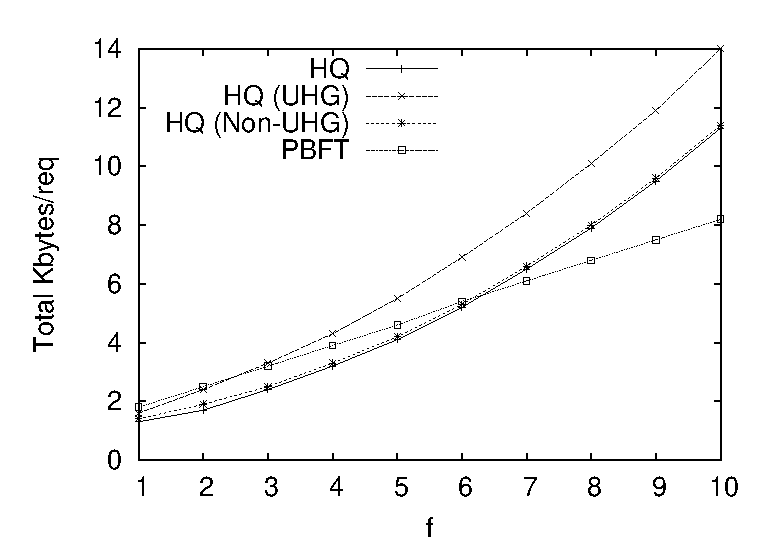
\includegraphics[width=3.0in]{analysis/byte-counts-Payload-256B.ps}
\caption{Comparing number of bytes processed per replica per client request. Request and reply
sizes are
256 bytes each.}
\label{fig:compare_bytes_256}
\end{figure}
\fi

\if 0
\begin{figure}
\centering
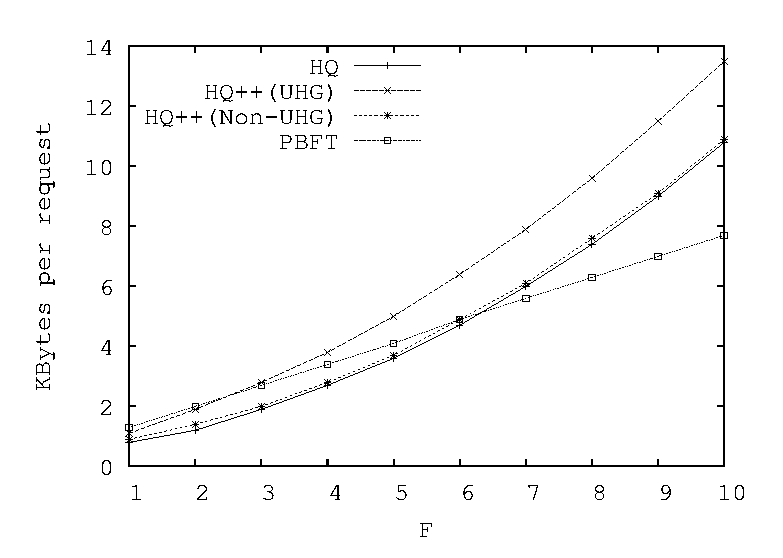
\includegraphics[width=3.0in]{analysis/compare-bytes-10-byte-req.ps}
\caption{Comparing number of bytes processed per replica per client request. Request and reply
sizes are 10 bytes each.}
\label{fig:compare_bytes_10}
\end{figure}
\fi

Figure~\ref{fig:compare_msg_counts} presents the number of messages processed per client 
request. Note that the load on UHG replica increases significantly compared to non-UHG replicas.


\if 0
\begin{figure}
\centering
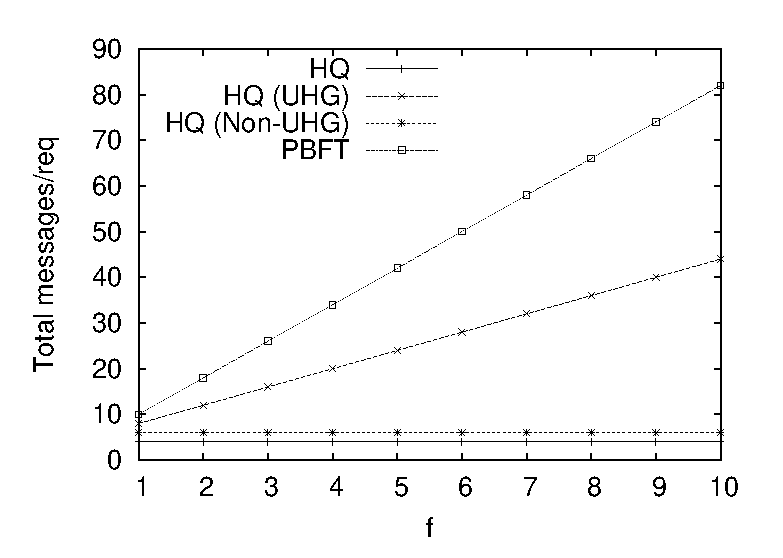
\includegraphics[width=3.0in]{analysis/message-counts.ps}
\caption{Comparing number of messages exchanged per replica per client request.}
\label{fig:compare_msg_counts}
\end{figure}
\fi


\paragraph{Summary} Is HQ under no contention better than PBFT (with batching = 1) at all
values of F? HQ's byte count increases quadratically due to the presence of certificates and 
therefore it becomes worse compared to PBFT at higher values of F. However, number of messages
exchanged is significantly less for HQ compared to PBFT. So, it really depends on how the 
transferring of bytes and processing of packets compare.
Interestingly, the HQ paper
compares for F $\le$ 5. 


\subsection{With batching}

PS-HQ can implement batching. UHG replica can send a sequence of hints in a single batchHint
message of the following schema: $\langle rid, seq, \langle cid, oid, op\#, ophash\rangle, 
mac\rangle$. In this hint, a vector of client requests are put together, as represented by the
vector in the batchHint. Ack for such hints are similar in schema and size. Size of
batch hint is: 4 + 4 + B * (4 + 4 + 4 + 20) + 20 = 28 + 32*B.

Under batching, replicas send a BatchWrite1OK message to one of the client who then sends a
BatcjWrite2 message. 
At this point, replicas execute the request and send a Write2-Ans to the individual
clients. 

Schema of BatchWrite1OK: $\langle rid, G \rangle$ where G is the batch grant. 

A batch grant has the following schema:
\\ $\langle rid, \langle cid, oid, op\#, ts\rangle, vs, hash,
auth\rangle$. Here, auth represents the authenticator, hash represents the hash of all operations
and inside array represents the timestamp each request gets. 

A batch certificate contains (2f+1) batch grants.

A client sends a BatchWrite message: $\langle cid, C\rangle$ where C is the batch certificate.


\paragraph{Number of protocol messages}

Figure~\ref{fig:compare_msg_counts_batching} shows the improvement of batching done
by the UHG replica and its impact on reducing the number of messages sent and
received.

Showing improvement on byte counts coming soon.....

\if 0
\begin{figure}
\centering
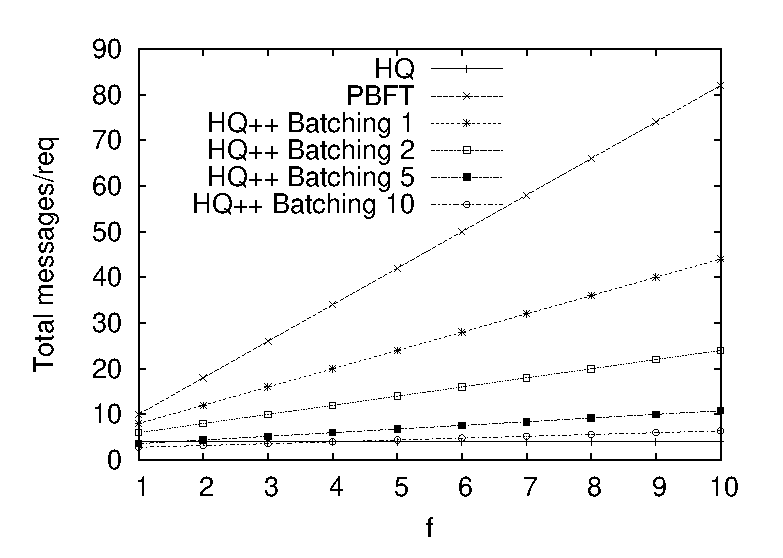
\includegraphics[width=3.0in]{analysis/message-counts-batching.ps}
\caption{Benefit of batching in terms of reducing the load on UHG replica.}
\label{fig:compare_msg_counts_batching}
\end{figure}
\fi




\subsection{Application benchmarks}

NFS for PS-HQ?, BI?

\subsection{PS-HQ}

\begin{itemize}
\item{}Vary contention to show how PS-HQ is better than HQ. \priority{High.}

\item{}Scale $f$ to identify which protocol is better: HQ, PBFT, PS-HQ. \priority{High}

\item{} How does a faulty pre-serializer affect things? \priority{High} \note{This may require
us to implement view change. However, we can avoid that by keeping the pre-serializer
different from the primary and hence the faulty pre-serializer simply
manifests itself as causing write conflicts.}
\item{} Batching. \priority{High}
\end{itemize}

\subsection{Protocol switching}

Vary workload characterisitics and show that the sytem works. \priority{Low}

\subsection{BI-HQ}
\begin{itemize}
\item{} With increasing $\alpha$, show the throughput and latency. \priority{High}
\item{} With increaing $f$. \priority{High}
\item{} Application? \priority{Medium?}
\item{} Under faults? \priority{Low}
\end{itemize}

\subsection{Divide and conquer (tentative)}

\subsection{Older Analytical Evaluation}
We use three metrics to compare different protocols: (i) response latency,
(ii) average number of messages processed by the replicas per client request, and (iii) 
average number of bytes processed by the replicas per client request.
We configure both PBFT and PS-HQ with batching size of 1. 


\stitle{Assumptions} We assume request and response payload of 256 bytes, TCP/IP header of 44 bytes,
8 byte MACs, 20 byte SHA-1 hash, 1 byte for client or replica ids, 4 bytes each for
the timestamps, sequence numbers and view identifiers.

\subsubsection{PS-HQ}
\stitle{Response latency}
HQ incurs 2 round trips or 4 message delays under normal case (i.e., no write contention and no
failurs). Contention resolution takes 4 additional message delays. 
PS-HQ incurs 5 message delays similarly to PBFT under no failures.

\stitle{Message load} Under no write contention and faults, average number of messages processed
by replicas in HQ is 4. Contention resolution protocol takes additional messages. Clients submit 
write contention certificate to the replicas. A quorum of replicas send the $\msg{Start}$ message
to the primary replica. Primary initiate the PBFT protocol, which incurs $8f$ additional messages 
on every replica. So, contention resolution adds $10f$ messages on the primary while $8f+2$ on the
non-primary replicas. The number of messages, on an average, as processed by a replica 
is given by $4+f\delta(14+16f)/(2f+1)$, where $\delta$ is the fraction of write requests that
required contention resolution. We assume that the validation for the requests is performed during
the last phase of the PBFT protocol, this avoids additional messages and delay for the HQ protocol.

PS-HQ incurs additional overhead on the hint generating replica compared to the HQ protocol: $2f$ messages
to be sent to the preferred quorum and receiving acknowledgements from the same quorum, a total
of $4+4f$ messages. Other replicas
receive 1 additional message from the hint generating replica and send an ACK to that replica compared 
to the HQ protocol, a total
of 6 message.
So, average message load of PS-HQ is $4+(12f/(2f+1))$. PBFT incurs message
load of $(8f+2)$. 

Figure~\ref{fig:abs_mesg_count_comp} compares HQ, PS-HQ and PBFT protocol according to the message
count. We observe two points: (i) HQ's message count approaches to that of PBFT as contention
increases, (ii) PS-HQ's message count is significantly lower than that of PBFT and is slightly
higher than HQ with no write contention.



\stitle{Byte load}
Figure~\ref{fig:byte_count_comp} compares the
bytes processed per client request for PBFT, HQ and PS-HQ protocol. We observe that
PS-HQ's overhead is slightly higher than HQ's overhead with no write contention, which is expected due
to the pre-serialization. However, PS-HQ incurs lower overhead than HQ under higher write contention.
HQ's overhead increases with write contention, surpassing the PBFT
protocol due to the additional work done by the HQ protocol before invoking the PBFT protocol and
the validation phase. PS-HQ incurs less overhead than PBFT because it offloads part of the work to
clients. Also, both PS-HQ and PBFT can implement batching, reducing the overheads further.

\if 0
\begin{figure}[t]
\centering
\begin{minipage}[t]{0.47\textwidth}
\scalebox{0.6}{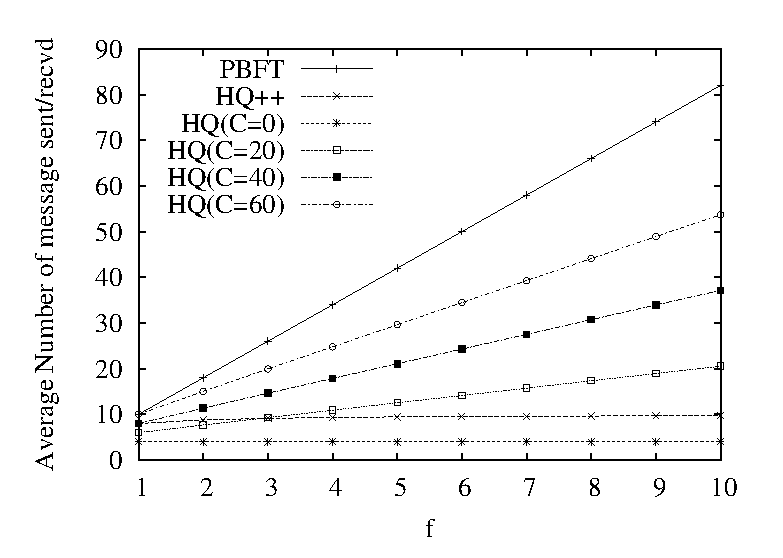
\includegraphics{graphs/Abs_Mesg_Count_Comp_PBFT_HQ}}
\caption{\label{fig:abs_mesg_count_comp} [\textbf{Pre-serialization}] Average message load.
$C$ represents contention in the workload.}
\end{minipage}
\begin{minipage}[t]{0.47\textwidth}
\scalebox{0.6}{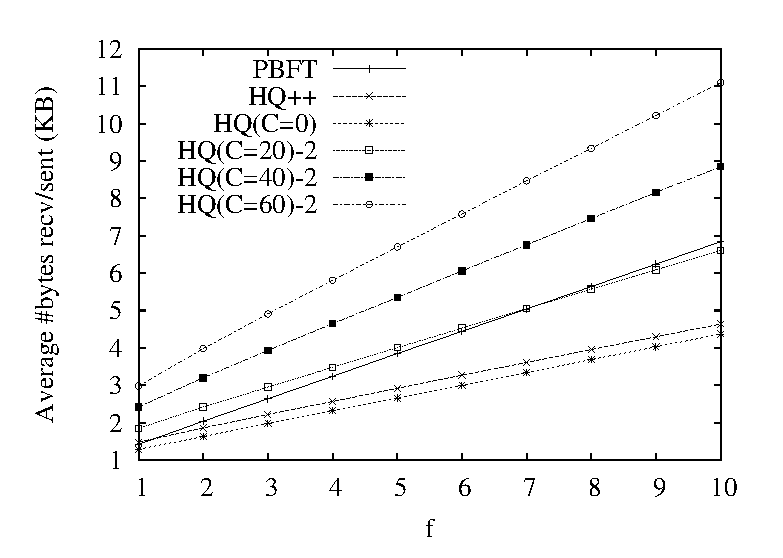
\includegraphics{graphs/Byte_Count_Comp}}
\caption{\label{fig:byte_count_comp} [\textbf{Pre-serialization}] Average byte load.}
\end{minipage}
\end{figure}
\fi

\stitle{Summary} Our analysis shows that HQ is superior to both PS-HQ and PBFT as long as there is
negligible write contention in the workload and both PS-HQ and PBFT do not implement high
batching. With higher write contention, PS-HQ is superior to both HQ and PBFT under fault free
settings and scales better with $f$.

\subsubsection{BI-PS-HQ}
Now, we consider the impact of relaxing the consistency requirements on the three metrics we
consider for comparision. We assume pre-integration of tentative updates before HQ is invoked
for linearization.

\stitle{Response latency} BI-PS-HQ completes requests in 2 message delays that do not cause replicas
to initate the synchronization phase. Requests that trigger a synchronization round require
4 additional message rounds. With numerical error set to $\alpha$, the average request
latency is $2+(4/\beta)$ message delays.

\stitle{Message load} Again, requests that do not trigger a synchronization round incur 2 messages.
Synchronization round requires replicas to send their tentative updates to
the pre-integrator replica, which waits to collect a quorum of such tentative updates and then 
invokes the HQ protocol. Overall, pre-integrator replica
incurs $8f$ additional messages during synchronization round: $2f$ for receiving a quorum of 
tentative updates, $2f$ to send the first phase
request, $2f$ to receive the response to first phase and $2f$ to write back. Non pre-integrator
replicas incur additional 4 messages during synchronization round. 
So, the average load is $2+(16f)/((2f+1)\beta)$. 
Figure~\ref{fig:mesg_comp_bi} compares BI-PS-HQ with PS-HQ and PBFT with increasing numerical error.
We set $\alpha= x.(3f+1)$ and vary $x$. This ensures that as $f$ scales, $\beta$ remains fixed
for a given $\alpha$ ensuring that synchronization round is triggered at a rate of $\beta$ and 
independent of $f$. We observe that the message
load on replicas drops in proportion to the relaxation in consistency: higher the $\alpha$, lower
the message count.  


\stitle{Byte load} 
Figure~\ref{fig:bytes_comp_bi_new} compares the byte load at replicas. 
Again, we observe that as consistency is relaxed, the byte count overhead of BI-PS-HQ 
drops proportionally. 

\if 0
\begin{figure}[t]
\centering
\begin{minipage}[t]{0.47\textwidth}
\scalebox{0.6}{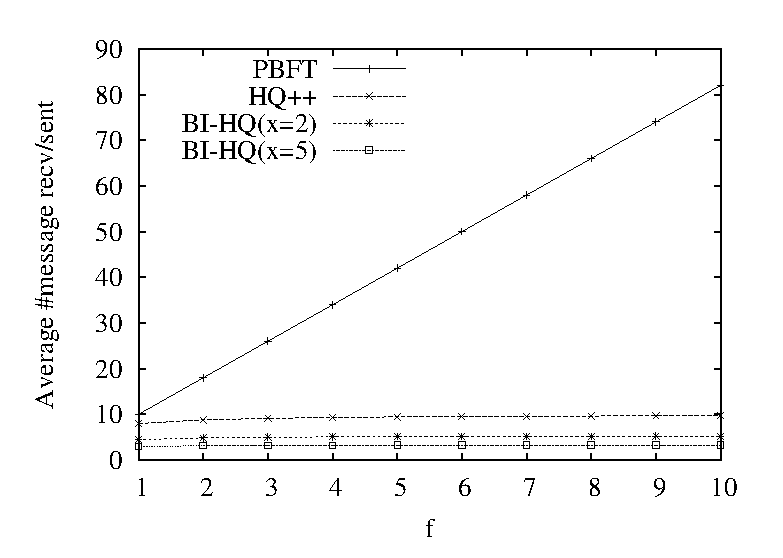
\includegraphics{graphs/Mesg_Count_Comp_BI_HQS}}
\caption{\label{fig:mesg_comp_bi}[\textbf{Relaxed Consistency}] Average message load.}
\end{minipage}
\begin{minipage}[t]{0.47\textwidth}
\scalebox{0.6}{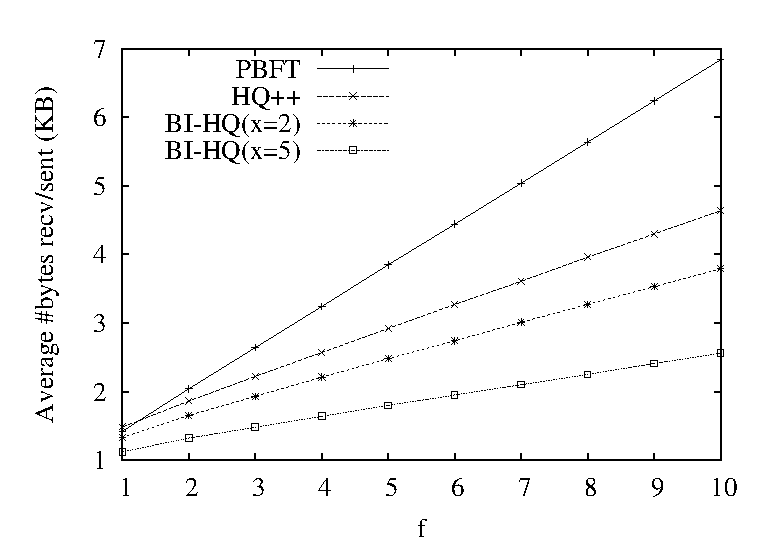
\includegraphics{graphs/Byte_Count_Comp_BI_New}}
\caption{\label{fig:bytes_comp_bi_new}[\textbf{Relaxing Consistency}] Average byte load.}
\end{minipage}
\end{figure}
\fi

\stitle{Summary} One can view BI-PS-HQ as PS-HQ configured with 
batching. Higher the relaxation in consistency, higher the batch sizes and hence lower the overhead. 
However, one important distinction
is that BI-PS-HQ does not sacrifice request latency whereas PS-HQ configured with higher batching increases
the request latency since hint generator has to wait to collect a batch of requests before initiating
the request processing.

\if 0
\begin{table}
\centering
\begin{tabular}{|c|c|c|c|c|}
\hline
\small{Metrics}& \textit{\small{PBFT}} & \textit{\small{HQ}} & \textit{\small{PS-HQ}} & \textit{\small{BI-PS-HQ}}\\
\hline
\hline
\textbf{\small{Latency}} & 5/2 & 2+$\delta$.7/2 & 5/2 &  1+$\frac{2}{\beta}$ \\
\hline
\textbf{\small{Load-Non-Primary}} & $\frac{8f}{k}$+2 & 4+(2+8$f$)$\delta$ & 6 & 2+$\frac{4}{\beta}$ \\
\hline
\textbf{\small{Load-Primary}} & $\frac{8f}{k}$+2 & 4+10$f\delta$ & 4+4$f$ & 2+$\frac{8f}{\beta}$\\
\hline
\textbf{\small{Average load}} & $\frac{8f}{k}$+2 & 4+$\frac{(14+16f)f\delta}{(2f+1)}$ & 4+$\frac{8f}{(2f+1)}$ &  2+$\frac{16f}{((2f+1)\beta)}$ \\
\hline
\textbf{\small{Load-Client}}& 4$f$+2& 9$f$+4& 9$f$+4 & 4$f$+2\\
\hline
\end{tabular}
\caption{Comparing the performance of different protocols with respect to the latency and message load.
 $\delta$ represents the fraction of contending writes (affects only the HQ protocol). k is the batch size for the PBFT protocol. }
\label{tab:overhead_est}
\end{table}

\fi

\section{Discussion}
\label{sec:analysis}
For an analytical comparison between PS-HQ, HQ, PBFT and BI-HQ, we assume failure free execution 
and use standard optimizations (preferred quorums, MACs, etc.). We present a summary of our
analysis due to space limitations, leaving the details to a technical report~\cite{hq++:website}. 

\stitle{1. PS-HQ vs HQ} PS-HQ adds one message delay to HQ and adds modest overhead for the
hint generator. However, under fault free executions, it avoids the contention 
resolution protocol whose
cost scales with $f$. Moreover, PS-HQ can implement batching. 
Therefore, we believe that PS-HQ is superior to HQ under fault-free settings.

\stitle{2. PS-HQ vs PBFT} Both PS-HQ and PBFT require 5 message delays to complete requests.
Both can implement batching. However, PS-HQ reduces the number of message exchanges significantly
since it does not require consensus. Moreover, PS-HQ offloads part of the work to clients, reducing
the overhead on replicas further. We therefore believe that PS-HQ scales better with $f$ compared to
PBFT.

\stitle{3. BI-HQ vs PS-HQ} BI-HQ completes requests in 2 message delays compared to 5 and 4
message delays with PS-HQ and HQ (under no conflicts) respectively. 
Protocol overhead of BI-HQ drops in proportion to the relaxation in consistency 
(i.e., higher $\alpha$  implies reduced overheads). One can view BI-HQ as PS-HQ with batching; higher
the inconsistency, higher the batch sizes. However, BI-HQ does not sacrifice request latency while 
PS-HQ (or PBFT) does with opportunistic batching.

Our initial experimental results have already confirmed
some of our expectations. For example, BI with PBFT provides request latency similar to a single round 
trip to $2f+1$ replicas on average,  as consistency is relaxed. 
\if 0
\begin{figure}
\centering
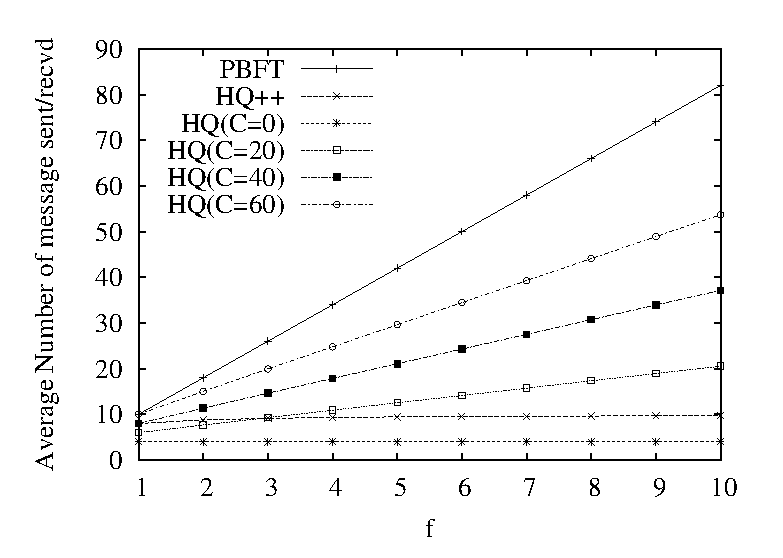
\includegraphics[width=3in]{graphs/Abs_Mesg_Count_Comp_PBFT_HQ}
\caption{\textbf{[Preserialization]} Average message load on replicas per client
request. $C$ represents the probability of conflicting writes in the workload.
}
\label{fig:abs_mesg_count_comp} \end{figure}

\begin{figure}
\centering
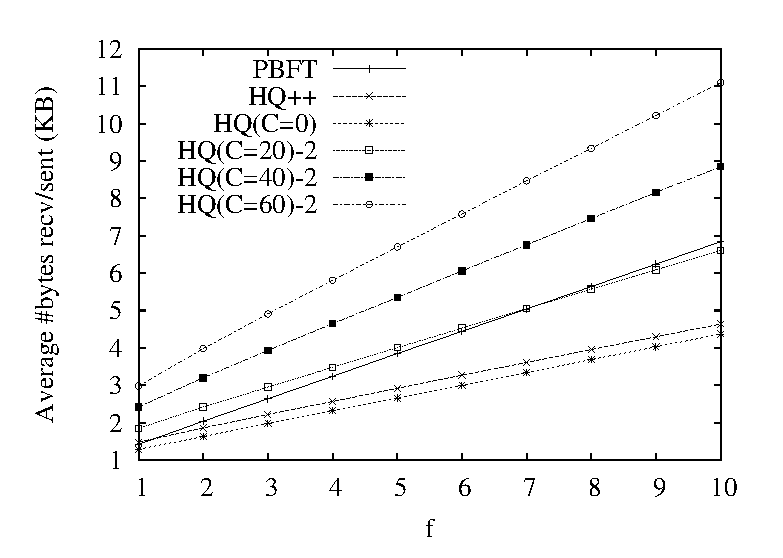
\includegraphics[width=3in]{graphs/Byte_Count_Comp}
\caption{\textbf{[Preserialization]} Average number of bytes sent and received (in KB) at replicas
per client request. Under contention, we assume
that only 2 write requests conflict (overhead increases further if more requests conflict).
}
\label{fig:byte_count_comp}
\end{figure}

\begin{figure}
\centering
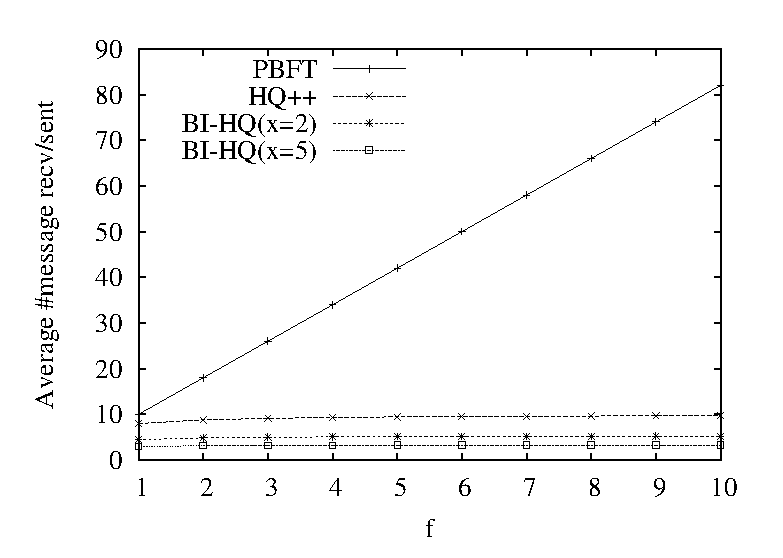
\includegraphics[width=3in]{graphs/Mesg_Count_Comp_BI_HQS}
\caption{\textbf{[Relaxed consistency]} Average message load on the replicas
per client request.
}
\label{fig:mesg_comp_bi}
\end{figure}

\begin{figure}
\centering
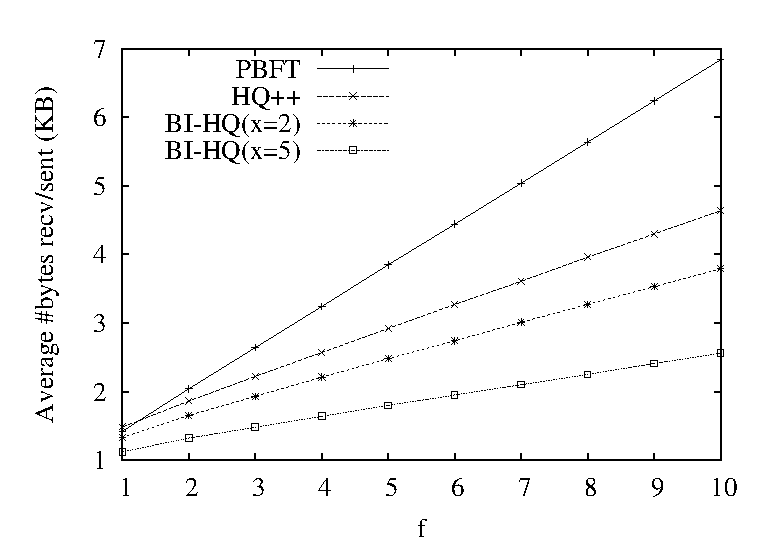
\includegraphics[width=3in]{graphs/Byte_Count_Comp_BI_New}
\caption{\textbf{[Relaxed consistency]} Average bytes (KB) sent/received by the replicas per client
request.
}
\label{fig:bytes_comp_bi_new}
\end{figure}

\fi

\if 0

\section{Related Work}

Say something about speculator~\cite{Speculator-sosp-05}.

Say something about relaxed consistency.

Say something about other, non-safe-hint optimizations of PBFT?

\fi






\if 0

\section{Appendix}

\stitle{Limitations?} Say something about limitations, e.g., that you
can't get drop-dead optimal performance without violating structuring
constraints.

\stitle{Trick applicability} Pre-serialization works for all quorum
systems, as long as we can infer the identity of the current
hint generator from the committed application state.
Bounded-inconsistency without pre-integration works for all BFT
systems.  Bounded-inconsistency with a pre-integrator works for all BFT
systems where the identity of the pre-integrator can be based on
committed state.


\stitle{Patterns and Reality} As with any system structuring pattern
(e.g., layering or the end-to-end principle), the safe hint pattern is
the launch pad, not the destination of a protocol designer's task.
Often further efficiencies can be obtained by violating the strict
boundaries of the pattern, typically at a great potential maintenance or
engineering cost.  In the case of BFT services, this boundary violation
also carries with it the need for extra validation effort, since now the
designers must prove the correctness properties for their entire design,
not just for the new components bracketing the original BFT system.  For
instance, the version of PS-HQ discussed in Section~\ref{sec:pshq} could
be made more efficient in terms of messages sent and message delays
required by combining the UHM with one of the replicas and leaving the
HQ client-replica protocol otherwise untouched.  Though this would not
change the reason for which PS-HQ performs better under contention, it
might further improve its overhead.  It would also, however, require a
rigorous proof that the modification to HQ does not invalidate its
guarantees.


\stitle{Further applicability} Other instances of safe hints.

Bells and whistles to the serializer (failure detector for
serializer)

Reducing load on serializer

Applications for \bihq

Systems such as Q/U, PBFT, and HQ are optimal for different areas
in the parameter space. For instance, for small replica sets, Q/U is
more efficient than HQ at low concurrency and PBFT is more efficient
than either at high concurrency. A fully adaptive systems would ideally
pick and choose which of Q/U, HQ, or PBFT (or their descendants and
competitors) to use according to a running estimate of the offered
workload. An untrusted protocol selector could perform that task. The
replica quorum executing the request stream arriving from the underlying
replicated state machine protocol could then validate the safety of the
request, as well as perhaps the safety of the choice of protocol based
on provable observations (e.g., a certificate of high recent concurrency
made of k concurrency certificates with timestamps within T values).

Undo during conflict resolution

Read requests.

hint generators for different objects (use h(view number, sequence
number, object ID) instead of h(view number, sequence number)).

hint generators chosen from the clients, not from the replicas?

Transactions.

Slow hint generators.


\begin{figure}
\centering
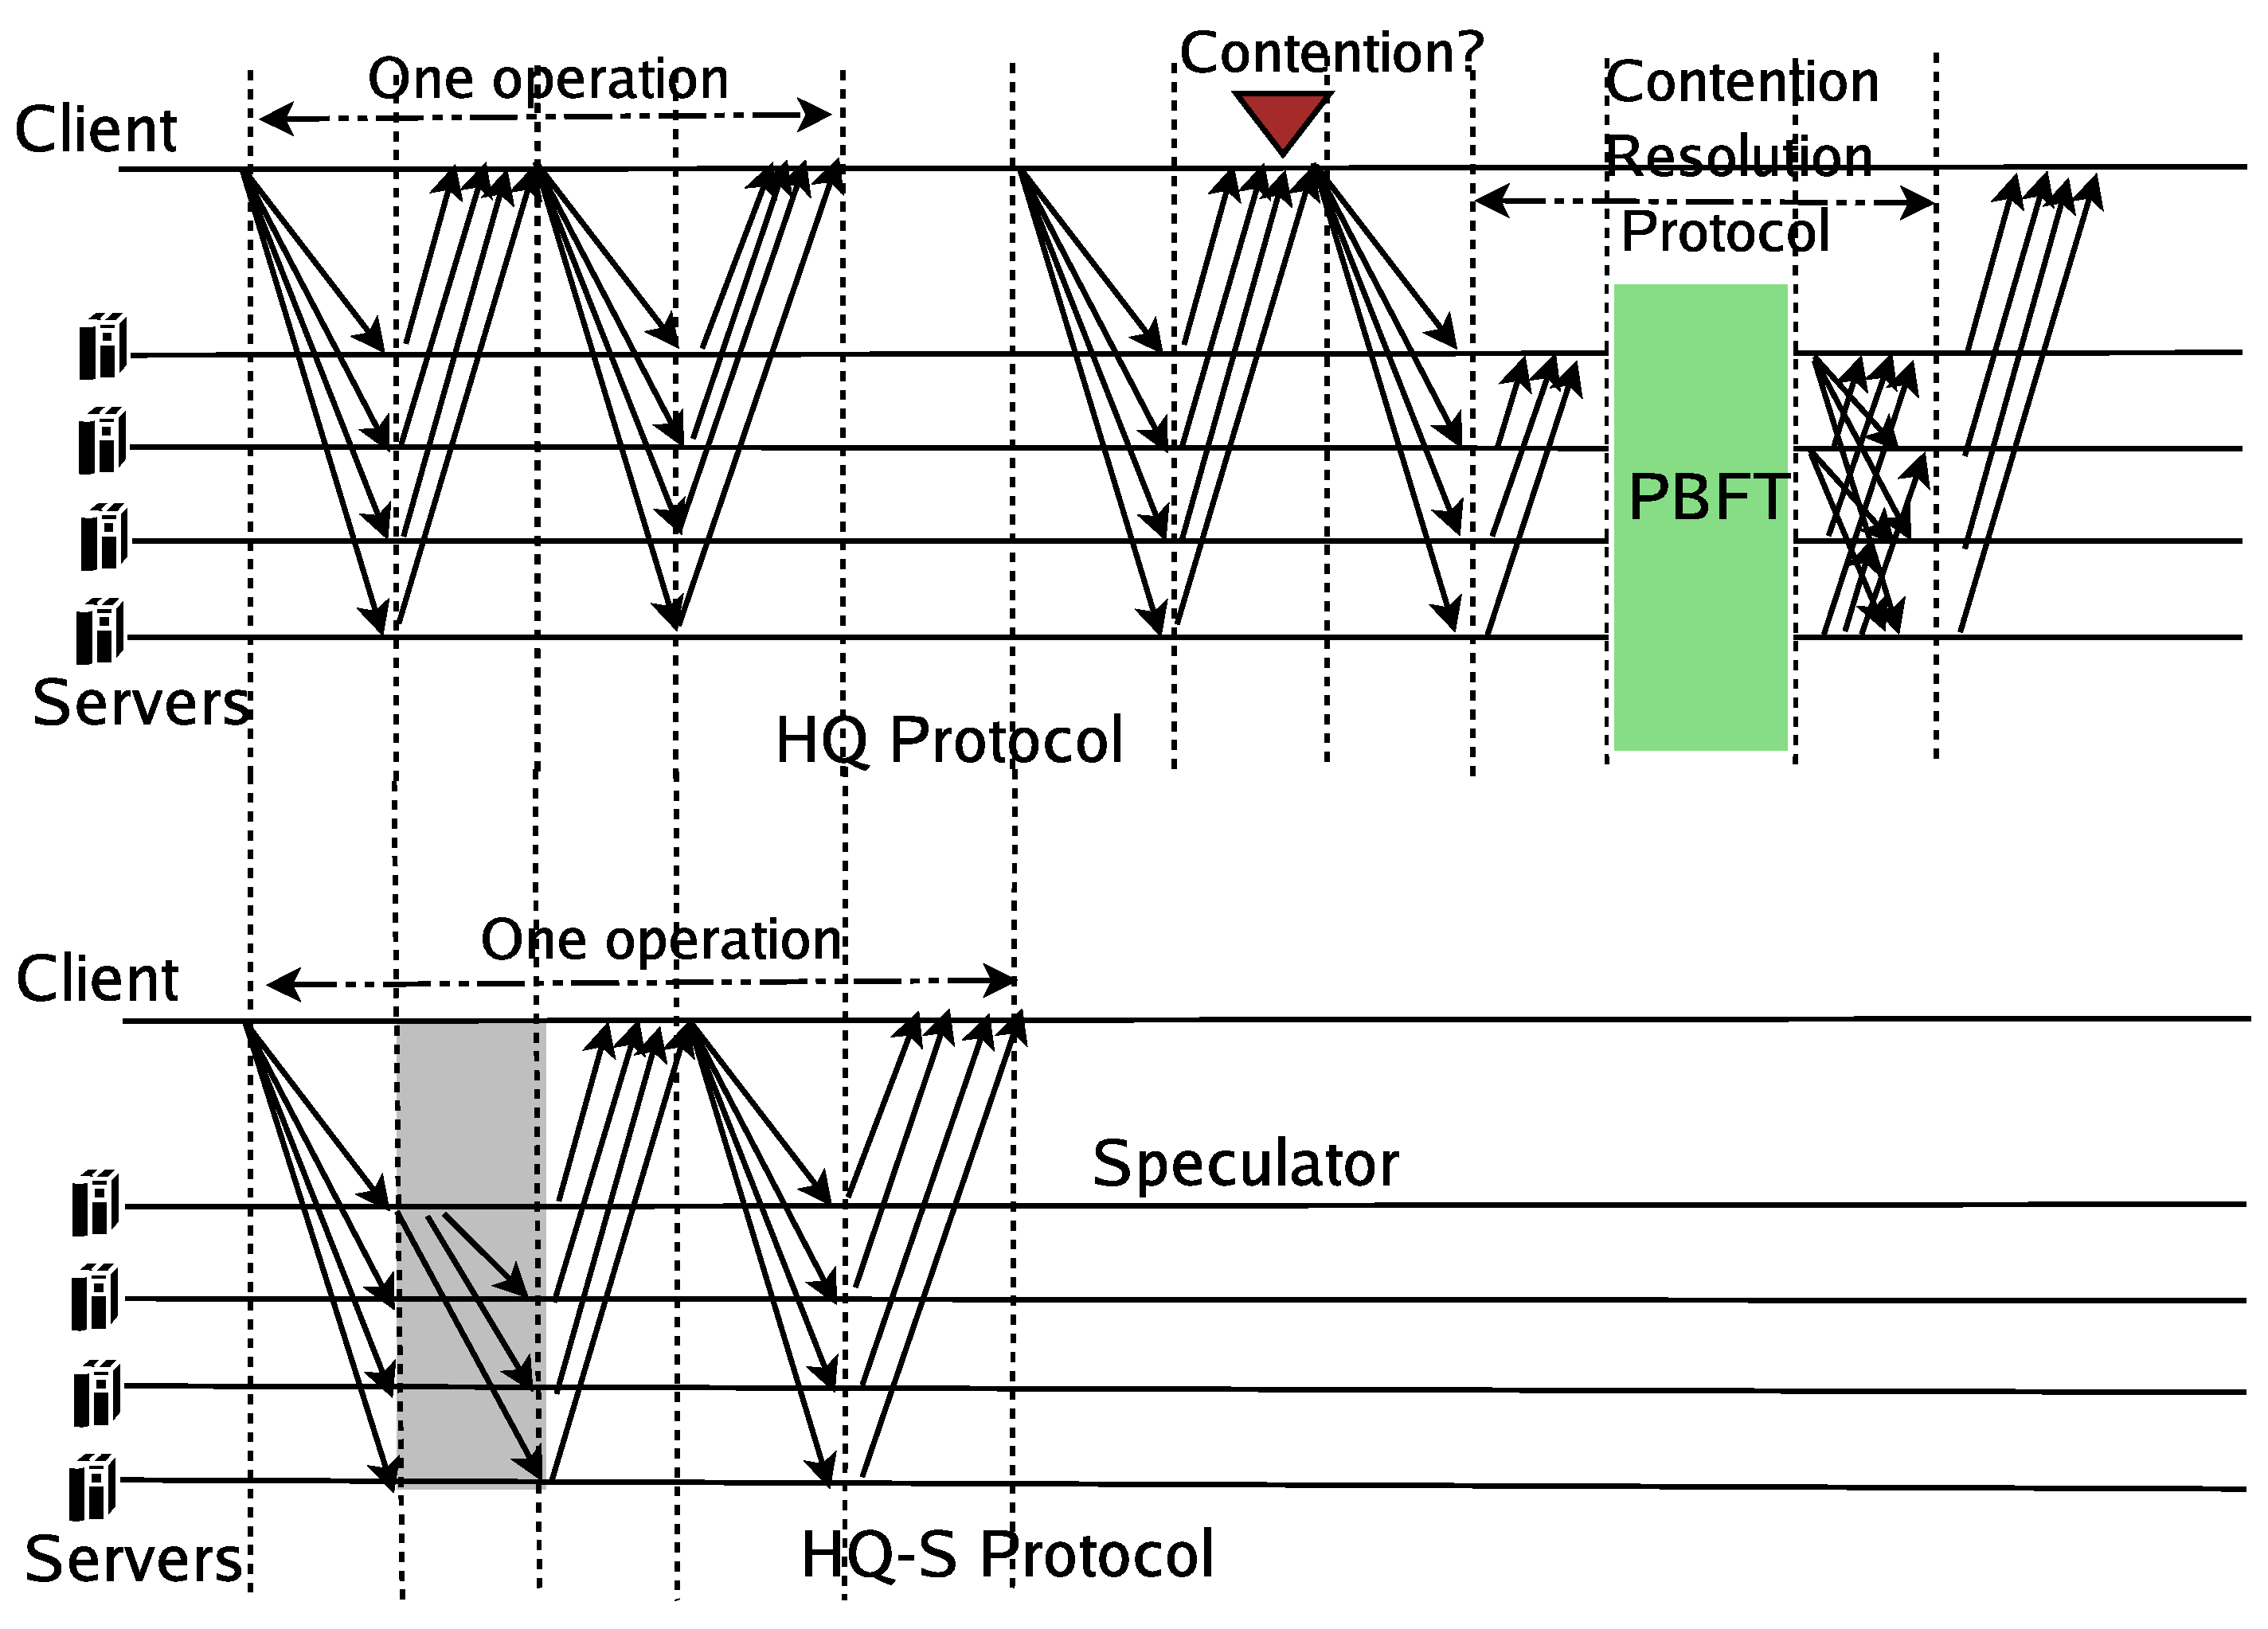
\includegraphics[width=3.2in]{hq++.eps}
\caption{Incorporating the hint generator in the HQ protocol. Note that PS-HQ
takes 5 message delays and HQ takes 4 message delays.  The extra delay is
due to the hint generator.}
\label{fig:pshq}
\end{figure}

Assumptions

Proof is provided in a separate technical report~\cite{}.

Many optimizations exist (e.g., second round of retransmission before
hint generator change, as with PBFT).



We are really great!


\fi





\if 0
\section{Target Applications}
\label{sec:applications}

\stitle{Key characteristics} Should be able to tolerated relaxed consistency.
Multiple writer. 

\stitle{Application that can tolerate weak consistency}
Here we identify the set of target applications that can benefit from the \bihq
protocol. So far we have:
\begin{itemize}
\item{} Domain Name System (DNS)
\item{} Checking invariants in distributed systems, such as content distribution networks (CDN's).
\item{} Routing Control Platform [NSDI'05]. 
\end{itemize}

\stitle{DNS} DNSSEC provides authentication to DNS but not widely used. DNS typically does not experience lot
of update/write workload. Majority of operations are queries. Some BFT based solutions have been proposed 
(from Liskov's group, not published) that tolerate faults in the nameservers. All nameservers are replicated to 
$3f+1$ replicas. The biggest problem with legacy DNS is the load on the nameservers higher up in the hierarchy.
Legacy DNS allows caching of DNS records and uses TTL for cache coherency. However, setting the right TTL is a burden
and introduces a tradeoff between overhead and coherency. This is true even for the BFT based DNS. There are some
proposals for a new DNS architecture (CoDoNS) which attempt to solve this problem via using an overlay to disseminate
updates in a timely fashion. \note{Need to think more on this one.}


\stitle{CDN} Publishers control membership, however need a mechanism to enforce certain invariants, e.g., 
each non-leaf member has taken at least a given number of children (control plane verification) and 
has forwarded sufficient number of data packets (data plane verification). \note{Again, need to think on this one.}

\stitle{RCP} RCP is a new proposal to deal with the complexity of identifying the optimal BGP paths for each 
router in an AS and to avoid the usual problems of routing loops being formed when distributed protocols are used, i.e., when
each router independently calcuates routes for itself. 
RCP obtains the full connectivity of the AS and the external BGP connectivity information to calculate such routes. However, a single 
RCP is problematic (single point of failure). Multiple RCP's needed to tolerate failure. However, what happens if some RCP's are faulty? 
(Consider for now that the routers are fault-free in the AS). Traditional BFT protocols can be used but there are opportunities to relax
the consistency requirements. First, routing protocols give best effort guarantee, so using a strict consistency BFT protocol
is probably an overkill. Moreover, since RCP is responsible for calculating the paths for every router in an AS, doing a BFT per
update and re-calculating the path for every router after such update is probably going to be too expensive. 
In fact, some router vendors do not reflect updates (of lower significance) immediately. 
They do it periodically. However the updates which affect the connectivity to tunnel endpoints are immediately reflected. 
This suggests that assigning different weights to different kind of updates can be used to identify when to do the BFT commit. 

\stitle{\bihq for RCP} Ideal state that RCP should achieve: each router's path is calculated instantly as soon as 
an update appears in the system. This is the ideal or 
strict consistency. Our goal is to relax this consistency. One idea: conit of each update is either the change in the link
weights (for link weight change updates) or some higher value if the link goes down. Numerical error is simply the weight of
such updates. This is fine, however its impact on usefulness of RCP is not clear. For example, can we answer a question like
this: at any time, what fraction of routes computed by RCP are optimal? What is its relationship with numerical error?
\fi













































\end{document}


%%%%%%%%%%%%%%%%%%%%%%%%%%%%%%%%%%%%%%%%%%%%%%%%%%%%%%%%%%%%%%%%%%%%
%%%%%%%%%%%%%%%%%%%%%%%  Moved the debugging junk here

\if 0

\subsection{Microbenchmarks: First set of emulab results}

\begin{figure}
\centering
\includegraphics[width=3.0in]{temp-Figures/throughput-hq.ps}
\caption{Throughput with HQ.}
\label{fig:throughtput-hq}
\end{figure}

\begin{figure}
\centering
\includegraphics[width=3.0in]{temp-Figures/throughput-hq++.ps}
\caption{Throughput with PS-HQ.}
\label{fig:throughtput-pshq}
\end{figure}



\begin{figure}
\centering
\includegraphics[width=3.0in]{temp-Figures/throughput-compare-hq-hq++.ps}
\caption{Comparing throughput of HQ with PS-HQ.}
\label{fig:throughtput-compare-hq-pshq}
\end{figure}


\subsubsection{Batching}

%\if 0
\begin{figure}
\centering
\includegraphics[width=3.0in]{temp-Figures/throughput-hq++-batching-f-1.ps}
\caption{Throughput with PS-HQ and batching at $f=1$.}
\label{fig:throughtput-hq-batching-f-1}
\end{figure}
%\fi
%\if 0
\begin{figure}
\centering
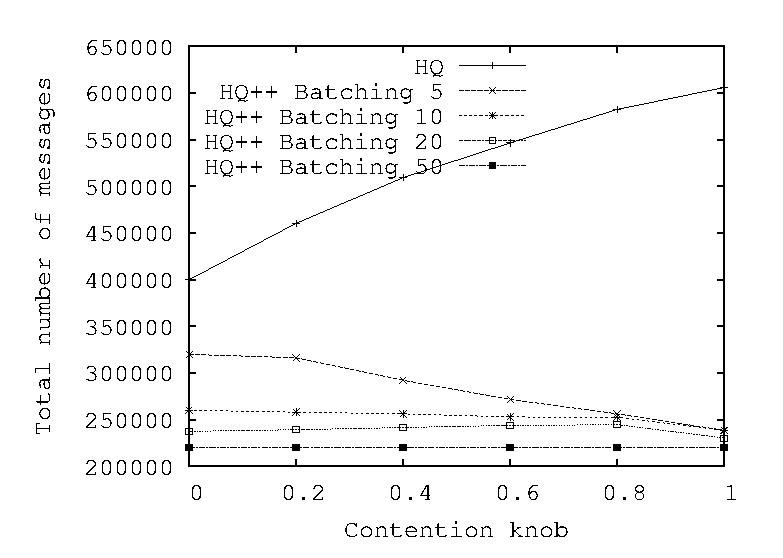
\includegraphics[width=3.0in]{temp-Figures/message-count-compare-batching-f-1.ps}
\caption{Comparing average number of messages processed with PS-HQ and batching at $f=1$.}
\label{fig:msg-count-hq-batching-f-1}
\end{figure}

\begin{figure}
\centering
\includegraphics[width=3.0in]{temp-Figures/traffic-compare-batching-f-1.ps}
\caption{Comparing average number of bytes processed with PS-HQ and batching at $f=1$.}
\label{fig:traffic-hq-batching-f-1}
\end{figure}


However, we observe from Figure~\ref{fig:throughtput-compare-hq-pshq} that at
no contention, PS-HQ's throughut is approx. 50\% of HQ. This is not good and we are trying to
identify the root cause of this behavior.


I ran an experiment on emulab with $f=1$ and measured the cpu utilization (via periodically
reading the /proc), memory consumed, total bytes send and received, elapsed time and bandwidth
for 100,000 operations. Results for the HQ case are similar across replicas. For the PS-HQ case,
I am presenting the results only for the preserializer replica. I had 20 clients, each 
has only one outstanding request at any given time.

Given a contention knob value, that fraction of requests generated by a client go to a 
shared object. Other requests go to a private object.


\paragraph{Points to note: 1} CPU utilization of PS-HQ is approx twice that of the HQ. This is
contrary to our expectation since PS-HQ never requires PBFT to invoke and hence our CPU
utitlization to be lower. In fact, at 0\% contention, we have significant CPU utilization (20\% 
or so). This definitely looks shady. My initial reaction is the part of the code base where
I insert the incoming requests and hints into a hashmap. The key of the hashmap is created
using some fields of the request. Any time a request arrives or a hint from the preserializer
arrives, I look up into the hashmap storing the hints or hashmap storing the requests. I dont think
this should be a problem since the number of requests we are talking about here is at most 20
at any given time and hence the time to lookup into the hashmap should be constant. Ideas?
Probably the insertions and deletions are causing the problem.

\paragraph{Points to note: 2} Network is not the bottleneck for this experiment as shown by
Figure~\ref{fig:bw}. As I was
mentioning in the telecon, for higher $f$, I was seeing throughput of 95Mbps. However, this
bandwidth does not seem to be a problem in this experiment. Finally, I am using HQ's method for
calculating the BW. I looked/asked around for hints about if Emulab has a facility to identify
the link utilization. There does not exist a simple mechanism to find that out. Basically, we
can ask emulab to tcpdump the packets and it will give us the dumps later. We can run our tests
to identify the bandwidth used and so on.

\paragraph{Points to note: 3} Figure~\ref{fig:mem} shows that PS-HQ consumes twice the memory. 
Even though the absolute values are
minute compared to the available memory, we need to identify why we are consuming twice. This
may hint at a bug probably. Figure~\ref{fig:bytes} shows that PS-HQ sends a fixed number of
bytes irrespective of the contention. The numbers also make sense given that both the request
size (approximately 60 bytes) and hint (adding hint and hintAck is approximately 60 bytes).
If we add the 20 bytes for the TCP/IP headers, then the numbers look consistent.
Since they are comparable in size, our relative overhead compared to HQ looks bad. At some
point, I will run experiment with higher request sizes.

\paragraph{Points to note: 4} Figure~\ref{fig:elapsed} shows the time taken to complete 
100,000 requests. This is essentially showing why PS-HQ is doing worse. Curve shows that the
elapsed time grows linearly with contention. As we know, with increasing contention, 
the request queue at the preserializer would increase and PS-HQ would behave as if serving to
a single client. I think the first validation check is to verify the throughput of PS-HQ
with single client and see if it matches what we are obtaining at 100\% contention. If it matches,
then we have to argue that indeed PS-HQ can not do better than PS-HQ with single client. 

\begin{figure}
\centering
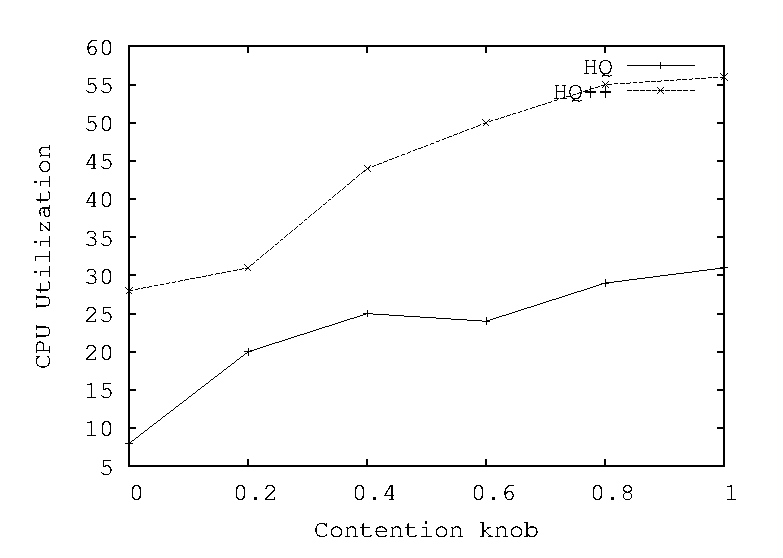
\includegraphics[width=3.0in]{temp-Figures/cpu.ps}
\caption{CPU Utilization}
\label{fig:cpu}
\end{figure}

\begin{figure}
\centering
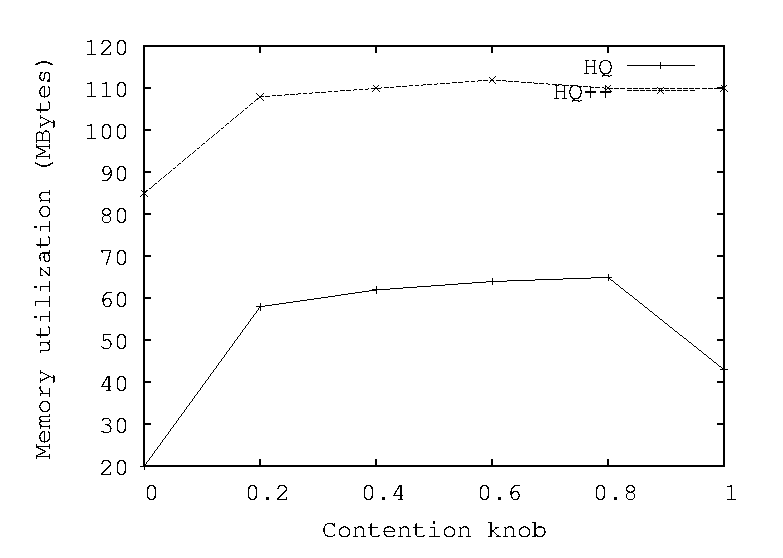
\includegraphics[width=3.0in]{temp-Figures/mem.ps}
\caption{Memory Consumed}
\label{fig:mem}
\end{figure}

\begin{figure}
\centering
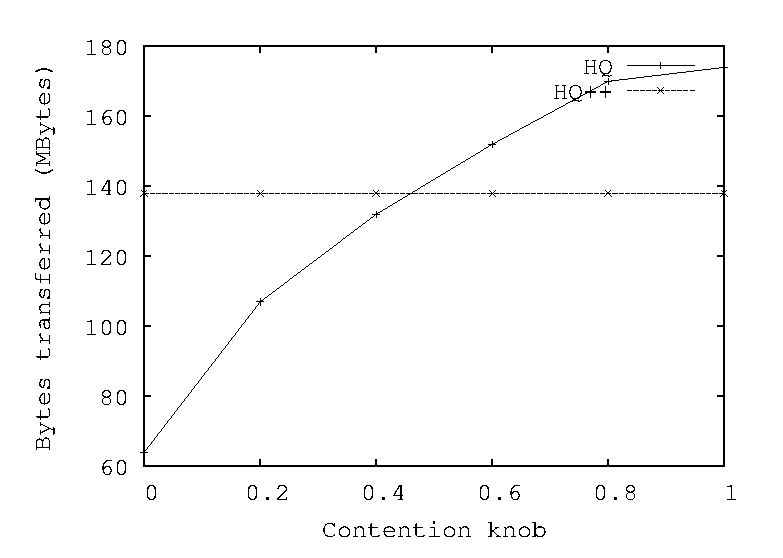
\includegraphics[width=3.0in]{temp-Figures/bytes.ps}
\caption{Total bytes send and received. }
\label{fig:bytes}
\end{figure}

\begin{figure}
\centering
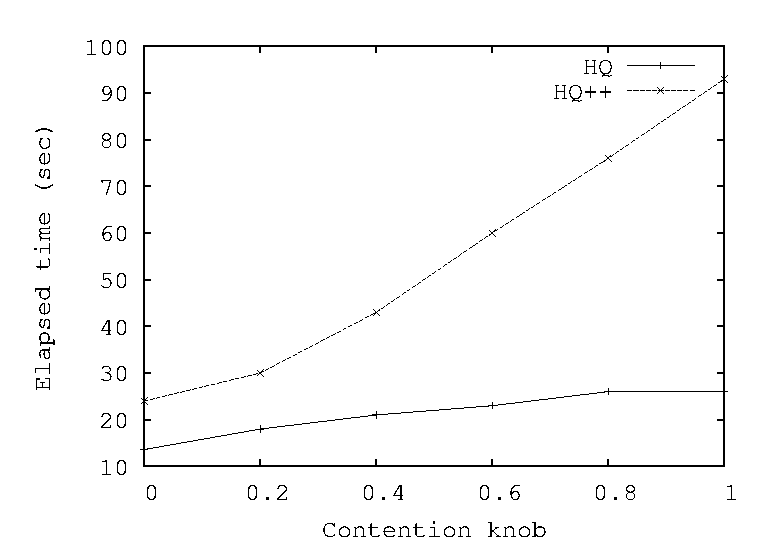
\includegraphics[width=3.0in]{temp-Figures/elapsed.ps}
\caption{Time needed to complete 100,000 operations.}
\label{fig:elapsed}
\end{figure}

\begin{figure}
\centering
\includegraphics[width=3.0in]{temp-Figures/bw.ps}
\caption{Bandwidth used. Basically = bytes/elapsed.}
\label{fig:bw}
\end{figure}



\fi
